\chapter{Introduction}\label{chap_intro}

The World Bank Group lends billions of dollars each year to fund development projects in its efforts to reduce global poverty. This project helps investigators at the Bank search for patterns of collusion, corruption, and fraud in its contracts data, using models of contract-specific risk. By developing an automated approach to detect these offenses this project can help the World Bank efficiently target future investigations.

Several things are required for a project of this type to achieve success \parencite{dssg_proj_list}. The following list outlines the requirements for a successful project, some requirements easier to satisfy so it is ordered from easiest to most difficult. These alone do not guarantee success, but success is nearly impossible without them.  \textit{A solvable problem}. This project cannot solve poverty, but it can help alleviate it by reducing corruption, collusion and fraud. 
\textit{A challenging problem}. Challenging problems encourage teamwork, spawn creative solutions, and play a key role in a Data Scientist's ability to solve real-world problems and an understanding, excitement, and passion for solving problems with social impact. For example, this World Bank project involved  search-engine expertise to find links between corrupt applicants online. 
\textit{An important problem with social impact}. Working in a big project is an investment, not only financially, but also opportunistically (when we choose to do a project, we choose not to do another project). It is important to dedicate the limited resources to substantial problems. Each project must meet an operational need for the partner organization and must have a tangible connection to ``social good.'' For example, this project helps more people over fewer people and that solve chronic problems over temporary problems. 
\textit{A motivated, capable, and committed partner}. No project can succeed without a fully invested project partner. Project partners understand the problem, they have subject-matter expertise, and they ultimately decide how a Data Scientist's work is used. Partners often look at the problem differently, which is important for solving tough problems.  Partners provide insight into the problem and to guide Data Scientist to develop a solution. This demands a lot from partners. It often requires partners stretching themselves and asking themselves hard questions. It also requires time. For this project, the World Bank helped scope the problem before it started, they gave a complete presentation about their work, they were available for at least once a week for feedback and discussion during the duration of the project, and they are actually using the results of this work when it finished. 
\textit{Appropriate, relevant data}. Getting the data a project  needs is almost always the biggest challenge. Important things go unmeasured or unrecorded or, more commonly, cannot be shared. Many projects involve  sensitive information. Getting lawyers to agree on data and code sharing can take months. It is important for Data Scientist to be flexible. Partners have anonymized data (while keeping it useful at an individual level), conducted background checks, and require Data Scientist to do analyses on their internal computer systems (remotely). All this while maintaining a spirit of openness.  In this case, the World Bank contributed with all the relevant data they have in order to build a solution that's appropriate, effective, and easily deployed.

\section{The World Bank}\label{sec_intro_wb}

The World Bank was created in 1944 as one institution and has evolved into an association of five development institutions. It is composed by  the International Bank for Reconstruction and Development (IBRD), the International Development Association, the International Finance Corporation (IFC), the Multilateral Guarantee Agency (MIGA), and the International Center for the Settlement of Investment Disputes (ICSID). In its interior it was formed by a large group of engineers and financial analysts who work from Washington, D.C. Now, they have a very heterogeneous and distinct staff that includes economist, public policy experts, sector experts and social scientists and about one third of the workers has spread to the country offices. They have more than 10,000 employees in more than 120 offices worldwide. While reconstruction remains an important part of their objectives, however, at today's World Bank, poverty reduction through an inclusive and sustainable glottalization remains the overarching goal. For details see \parencite{wb_history}. 

The World Bank Group has set two goals for the world to achieve by 2030; first, end extreme poverty by decreasing the percentage of people living on less than \$1.90 a day to no more than 3\%; second, promote shared prosperity by fostering the income growth of the bottom 40\% for every country; third, the World Bank is a vital source of financial and technical assistance to developing countries around the world. The World Bank Group is not a bank in the ordinary sense but a unique partnership to reduce poverty and support development. \parencite{wb_about}

The World Bank Group provides Financial Products and Services by giving out low-interest loans, zero to low-interest credits, and grants to developing countries. ``These support a wide array of investments in such areas as education, health, public administration, infrastructure, financial and private sector development, agriculture, and environmental and natural resource management. Some of our projects are cofinanced with governments, other multilateral institutions, commercial banks, export credit agencies, and private sector investors.''\parencite{wb_about}. They offer financing through trust fund partnerships with bilateral and multilateral donors. For example, many partners have asked the Bank to help manage initiatives that address needs across a wide range of sectors and developing regions.

This work focuses in these Financial Products and Services. It analyzes their contracts (SEE CHAP XXXXXX) by using historical data on over 300,000 major contracts funded by World Bank in the form of low-interest loans, zero to low-interest credits, and grants to developing countries covering  from the past 20 years. Historical data including such features as company name, country, sector, and total award amount.

The World Bank also provides Innovative Knowledge Sharing, by offering support to developing countries through policy advice, research and analysis, and technical assistance. ``The analytical work often underpins World Bank financing and helps inform developing countries' own investments. In addition, we support capacity development in the countries we serve. We also sponsor, host, or participate in many conferences and forums on issues of development, often in collaboration with partners.''\parencite{wb_about}

This is why this project becomes of high value for the World Bank Group. On one hand, this work helps them to provide much better Financial Products and Services by reducing the cost that corruption, collusion and fraud generates in the process of lending money to developing countries throughout the world's developing countries. On the other, this project contribute to their Innovative Knowledge Sharing by supplying them with the necessary tools and algorithms they need in order to share corruption, collusion and fraud analysis' results.

This project relies on the fact that the World Bank group, in order to ensure that countries can access the best global expertise and help generate cutting-edge knowledge, is constantly seeking to improve the way it shares its knowledge and engages with clients and the public at large. This includes  measurable results, improving every aspect of their work like how projects are designed, how information is made available, and how to bring our operations closer to client governments and communities and also includes  their Open Development, a set of free, easy-to-access tools, research and knowledge to help people address the world's development challenges. This work would not be possible without all this previous work and is a virtuous circle because it contributes by helping them achieve this goal.

This work uses the Open Data\footnote{Go to \cite{wb_data}} website from the World Bank, which offers free access to comprehensive, downloadable indicators about development in countries around the globe, data needed in order to detect and predict patterns of collusion, corruption, and fraud in its contracts data by using models of contract-specific risk. 

\section{The Wold Bank Group's Rules and Guidelines}

The process by which the World Bank Group gives out low-interest loans, zero to low-interest credits, and grants to developing countries is not simple. They have a set of guidelines available online \parencite{wb_g_proc} in which they specify how to apply to all the contracts for goods, works and services financed in whole or in part from the Bank's loans, credits and grants which would thereby cover both IBRD and IDA. Similar provisions apply for the selection of Consultants under the Consultants Guidelines \parencite{wb_g_cons}. For the purpose of this project the Consultants will not be deeply explained. 

In the World Bank's rules and guidelines they consider ``goods'' and ``works'' all the related services such as transportation, insurance, installation, commissioning, training, and initial maintenance. Also,  ``goods'' includes commodities, raw material, machinery, equipment, vehicles, and industrial plant. 

``This requirement is made applicable in each operation through the loan, credit or grant agreement thus making their use a legal obligation on the part of the Borrower. It applies as well to counterpart funds that are also used to finance contracts with loan/credit proceeds. In addition, parts of Bank-financed projects that are co-financed by other donors are also subject to Bank rules. This could also be the case under parallel financing when co-financiers agree to using Bank guidelines (leverage effect).''\parencite{wb_rules}

In order to ensure that these legal provisions are observed during project implementation, Bank staff review and provide a ``no objection'' before the Borrower implements certain procurement decisions\footnote{For all International Competitive Bidding (ICB) and other high-value, high-risk, and otherwise complex contracts}. Bank staff will review all the contracts that have not been subject to Prior Review so as to ensure that the Guidelines were applied as required. Where this is found not to be the case, the Bank applies various remedies including \textit{mis-procurement}, which in most instances requires cancellation and refund of the funds in question\footnote{Advertising requirements vary depending on whether Procurement is subject to International Competitive Bidding (ICB) or National Competitive Bidding(NCB).}.

\subsection{Procurements General Considerations}

In every Procurement the World Bank expect that the responsibility for the implementation of the project, and therefore for the award and administration of contracts under the project, rests with the Borrower. The Bank, is required ensure that the proceeds of any loan are used only for the purposes for which the loan was granted, with due attention to considerations of economy and efficiency and without regard to political or other non-economic influences or considerations. While in practice the specific procurement rules and procedures to be followed in the implementation of a project depend on the circumstances of the particular case, four considerations generally guide the Bank's requirements:
\begin{enumerate}[a)]
\item ``the need for economy and efficiency in the implementation of the project, including the procurement of the goods, works, and non-consulting services involved;
\item the Bank's interest in giving all eligible bidders from developed and developing countries the same information and equal opportunity to compete in providing goods, works, and non-consulting services financed by the Bank;
\item  the Bank's interest in encouraging the development of domestic contracting and manufacturing industries in the Borrowing country; and
\item the importance of transparency in the procurement process.''\footnote{See \cite{wb_g_proc}.}
\end{enumerate}

The World Bank's guidelines for procurement of goods, works, and non-consulting services \parencite{wb_g_proc} establishes that open competition is the basis for efficient public procurement.  In their articles, they state that each Borrower shall select the most appropriate method for the specific procurement. They have to choose between International Competitive Bidding (ICB) on National Competitive Bidding (NCB). This means, in most cases, ICB, properly administered, and with the allowance for preferences for domestically manufactured goods and, where appropriate, for domestic contractors for works under prescribed conditions is the most appropriate method. The Bank requires its Borrowers to obtain goods, works, and non-consulting services through ICB open to eligible suppliers, service providers, and contractors\footnote{Section II of these Guidelines describes the procedures for ICB \parencite{wb_g_proc}.}.

In order to satisfy these requirements, any procurement needs to be transparent, competitive and legal according to the guidelines the World Bank established. Contractors providing goods and services on World Bank projects are typically hired through a competitive bidding process. The problem is that in practice, the Borrowers and Contractors tend not to fulfill those requirements. Occasionally, prospective contractors influence the competitive system by colluding with other contractors, bribing government officials, or otherwise manipulating the bidding process. These offenses have far-reaching effects on the price and quality of contract delivery.  There is a considerable amount of cases in which corruption, collusion and/or fraud takes place. The guidelines include some sections to address those problems. The World Bank is committed to detecting instances of collusion, corruption, and fraud in order to maximize its global impact.

\section{Corruption, Collusion and Fraud}\label{sec_intro_corruption}

The World Bank's guidelines for procurement of goods, works, and non-consulting services \parencite{wb_g_proc} establishes what's to be understood by corruption, collusion, fraud, coercion and obstruction. 

It is the Bank's policy to require that Borrowers\footnote{including beneficiaries of Bank loans.}, bidders, suppliers, contractors and their agents\footnote{whether declared or not.}, sub-contractors, sub-consultants, service providers or suppliers, and any personnel thereof, observe the highest standard of ethics during the procurement and execution of Bank-financed contracts. In pursuance of this policy, the Bank defines, the terms set forth below as follows\footnote{Definitions taken from \cite{wb_g_proc}. Updated to 2011.}:

\begin{definition}\label{def_corruption}
A \textit{corrupt practice} is the offering, giving, receiving, or soliciting, directly or indirectly, of anything of value to influence improperly the actions of another party.
\end{definition}

\begin{definition}\label{def_collusion}
A \textit{collusive practice} is an arrangement between two or more parties designed to achieve an improper purpose, including to influence improperly the actions of another party.
\end{definition}

\begin{definition}\label{def_fraud}
A \textit{fraudulent practice} is any act or omission, including a misrepresentation, that knowingly or recklessly misleads, or attempts to mislead, a party to obtain a financial or other benefit or to avoid an obligation.
\end{definition}

\begin{definition}\label{def_coersion}
A \textit{coercive practice} is impairing or harming, or threatening to impair or harm, directly or indirectly, any party or the property of the party to influence improperly the actions of a party.
\end{definition}

\begin{definition}\label{def_obstruction}
A \textit{obstructive practice} is deliberately destroying, falsifying, altering, or concealing of evidence material to the investigation or making false statements to investigators in order to materially impede a Bank investigation into allegations of a corrupt, fraudulent, coercive or collusive practice; and/or threatening, harassing or intimidating any party to prevent it from disclosing its knowledge of matters relevant to the investigation or from pursuing the investigation, or acts intended to materially impede the exercise of the Bank's inspection and audit rights.
\end{definition}

In its effort to avoid practices from definitions \ref{def_collusion} to \ref{def_obstruction}, the World Bank
will respond accordingly to each contract in question. 
The Bank will \textit{reject a proposal} for award if it determines that the bidder recommended for award, or any of its personnel has, directly or indirectly, engaged in corrupt, fraudulent, collusive, coercive, or obstructive practices in competing for the contract in question. 
The Bank will \textit{declare mis-procurement} and cancel the loan if it determines at any time that representatives of the Borrower engaged in  any corrupt, fraudulent, collusive, coercive, or obstructive practices during the procurement or the implementation of the contract. 
The Bank will \textit{sanction} a firm or individual, including by publicly declaring such firm or individual ineligible, either indefinitely or for a stated period of time to be awarded a Bank-financed contract; and to be a nominated sub-contractor of an otherwise eligible firm being awarded a Bank-financed contract.
The Bank will require that a clause be included to permit the Bank to inspect all accounts, records, and other documents relating to the submission of bids and contract performance, and to have them audited by auditors appointed by the Bank.

The World Bank has a long history of giving loans for procurement of goods, works, and non-consulting services based on the four considerations listed above. As expected, there has been a long history of malicious activity in the procurements. This is why they publish a list of contractors which had been discovered to have a practice that lead to either a rejection, a mis-procurement, an obstructive practice or a sanction. This project refers to this list as the debarment data.

\subsection{World Bank Listing of Ineligible Contractors}

The World Bank publishes online \parencite{wb_debarment} a list that includes all the firms and individuals listed as ineligible to be awarded a World Bank-financed contract for the periods indicated because they have been sanctioned under the Bank's fraud and corruption policy as set in the Procurement Guidelines or the Consultant Guidelines.  Such sanction was imposed as the result of an administrative process conducted by the Bank that permitted the accused firms and individuals to respond to the allegations\footnote{``Through July 2007, this process was conducted in accordance with the Sanctions Committee Procedures adopted on August 2, 2001. Since then, the process has been conducted in accordance with the Sanctions Procedures of the World Bank Group Sanctions Board.''}, or a cross-debarment\footnote{ Since 2011.} made effective by the World Bank, Asian Development Bank, European Bank for Reconstruction and Development, Inter-American Development Bank, and African Development Bank.

The table \ref{tab_debarred_sam} bellow shows a short sample of how is the debarments list published. As it can be seen from the table \ref{tab_debarred_sam}, it includes a \textit{Firm Name, Address, Country, Inegibility Period} and \textit{Grounds}. The \textit{Firm Name} can be a person or an entity, the \textit{Ineligibility period} correspond to the time frame in which that specific \textit{Firm Name} is debarred from receiving any type of award financed by the World Bank, and finally, the \textit{Grounds} refers to the violations made to the Consultants Guidelines (CG) or the Procurements Guidelines (PG) and their specific article and section.

\begin{table}[H]
\caption{Debarred Firms and Individuals (sample)}
\label{tab_debarred_sam}
\resizebox{\textwidth}{!}{
\begin{tabular}{lrrccr}
\hline
\hline
\multirow{2}{*}{Firm Name} & 	\multirow{2}{*}{Address} & \multirow{2}{*}{Country}	& \multicolumn{2}{c}{Ineligibility Period} & \multirow{2}{*}{Grounds} \\ \cline{4-5}
 & & & From & To & \\
\hline
MR. NGUYEN & TOWER CENTER  & Vietnam& 15-DEC-2015 &	14-DEC-2026	& CG, 1.22(a)(ii); PG, 1.14(a)(ii)-(iii) \\
 PHUONG & OFFICE   &  &  & &\\
 QUY*298 &BUILDING,NO.  &  & & & \\
 &83A LY THUONG  &  & & & \\
 &KIET  &  &  & &\\
 &STREET,DISTRICT & &  &  & \\
 &HOAN KIEM,  HANOI & & &  & \\

SFC VIETNAM  & TOWER CENTER & Vietnam & 15-DEC-2015	& 14-DEC-2025 &	CG, 1.22(a)(ii); PG, 1.14(a)(ii)-(iii) \\
INVESTMENT & OFFICE  &  &  & &\\
DEVELOPMENT & BUILDING, NO.  &  &  & &\\
FOR ENVIRONMENT& 83A LY THUONG  &  &  & &\\
CORPORATION*297& KIET STREET,  &  &  & &\\
& DISTRICT HOAN  &  &  & &\\
& KIEM,  HANOI	 &  &  & & \\

MR. NIKOLAI & ANTONIENKO 3,-43,	& Russian & 	30-OCT-2015	& 29-OCT-2019	& CG, 1.22(a)(i) \\
GEORGIEVITCH  &  190000 SAINT  &  Federation &  & &\\
OBRADOVITCH*296 & PETERSBURG    &  &  & &\\
\hline
\hline
\end{tabular}
}
\footnotesize{\textbf{Source:} see the \cite{wb_debarment}.\\ \textbf{Notes:} Several firms above are marked with an asterisk (*). The period of ineligibility of the sanctioned firm extends to any firm directly or indirectly controlled by the sanctioned firm.}
\end{table}


The World Bank also publishes a second list that includes the \textit{Other Sanctions} that includes firms that are typically under a \textit{Conditional Non-debarment}. ``The Conditional Non-debarment means that so long as the sanctioned entity meets certain conditions, including (a) implementing a corporate compliance program acceptable to the Bank; (b) fully cooperating wtih the Bank; and (c) not attempting to evade the sanction imposed on the firm and those entities it directly or indirectly controls, the sanctioned entity will continue to be eligible to participate in Bank-financed activities.''\parencite{wb_debarment}; or has a \textit{Letter of Reprimand} by which the World Bank officially notifies the firm its sanction.


\section{Searching for \textit{red-flags}}

\begin{figure}[H]
\begin{center}
\caption{What does corruption look like?}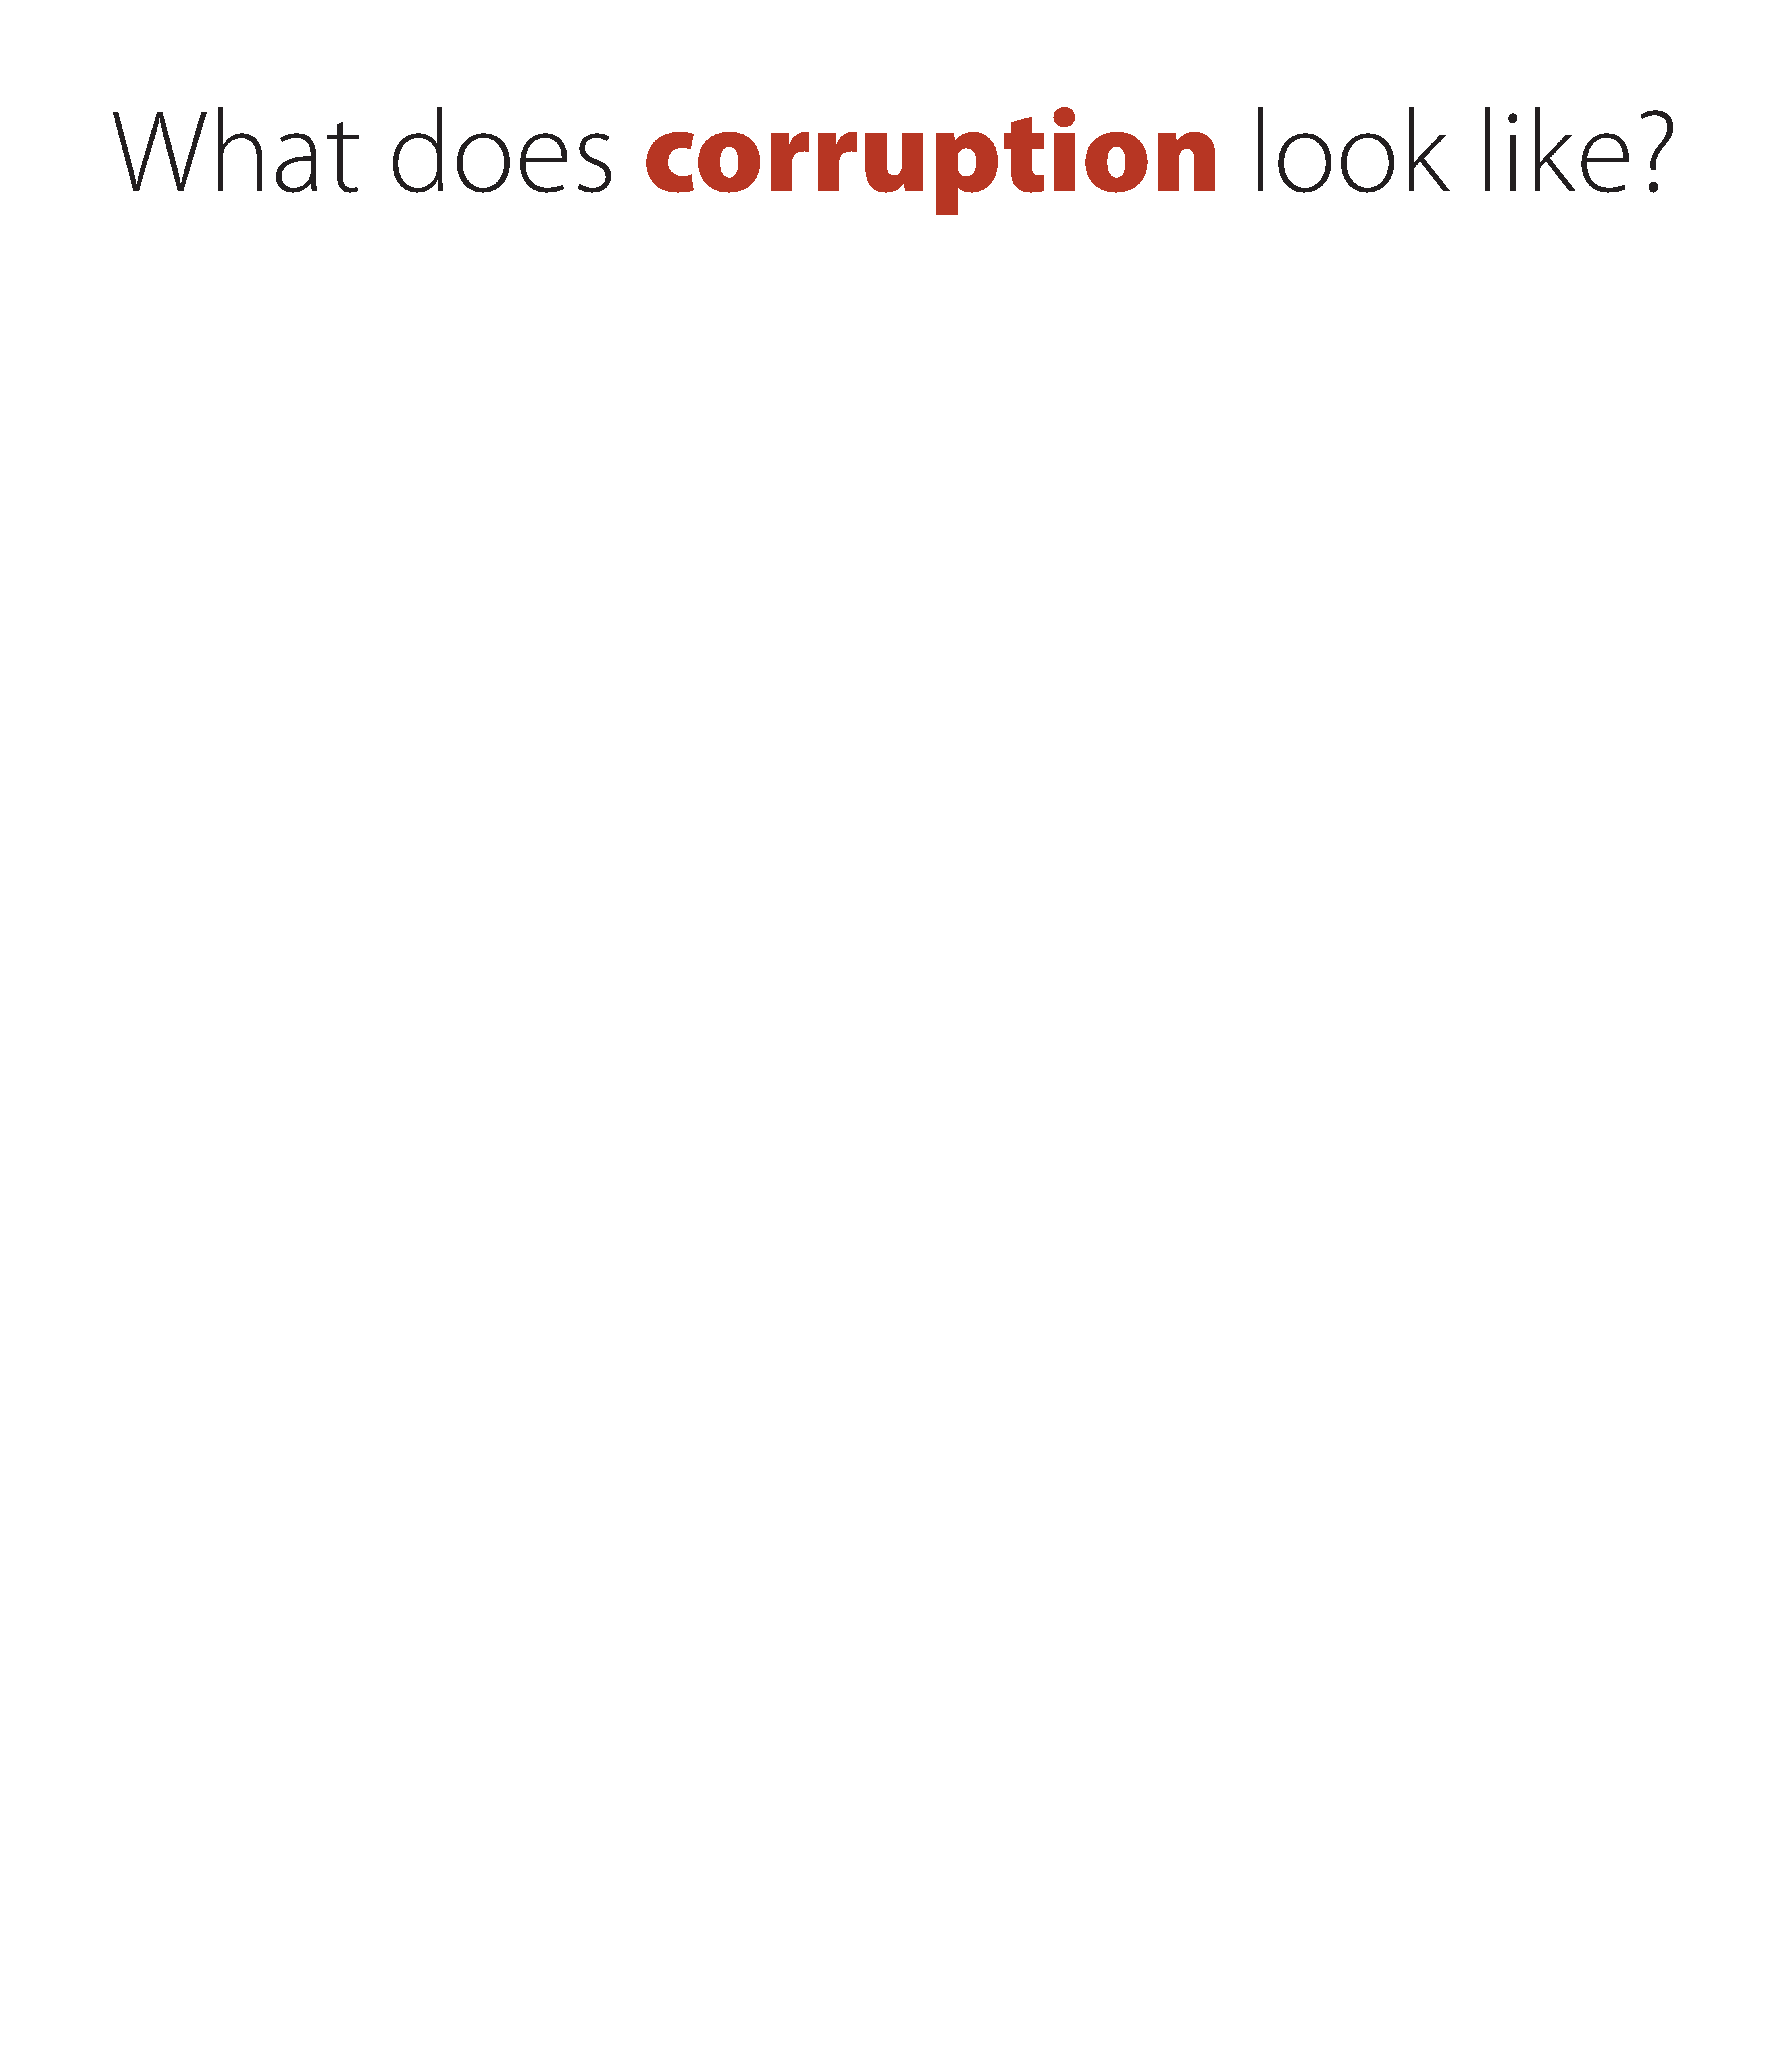
\includegraphics[max width=0.6\textwidth]{../img/poster_what.pdf}
\end{center}


\begin{subfigure}[t]{0.5\textwidth}
\caption{Cumulative value of non-competitive contracts}
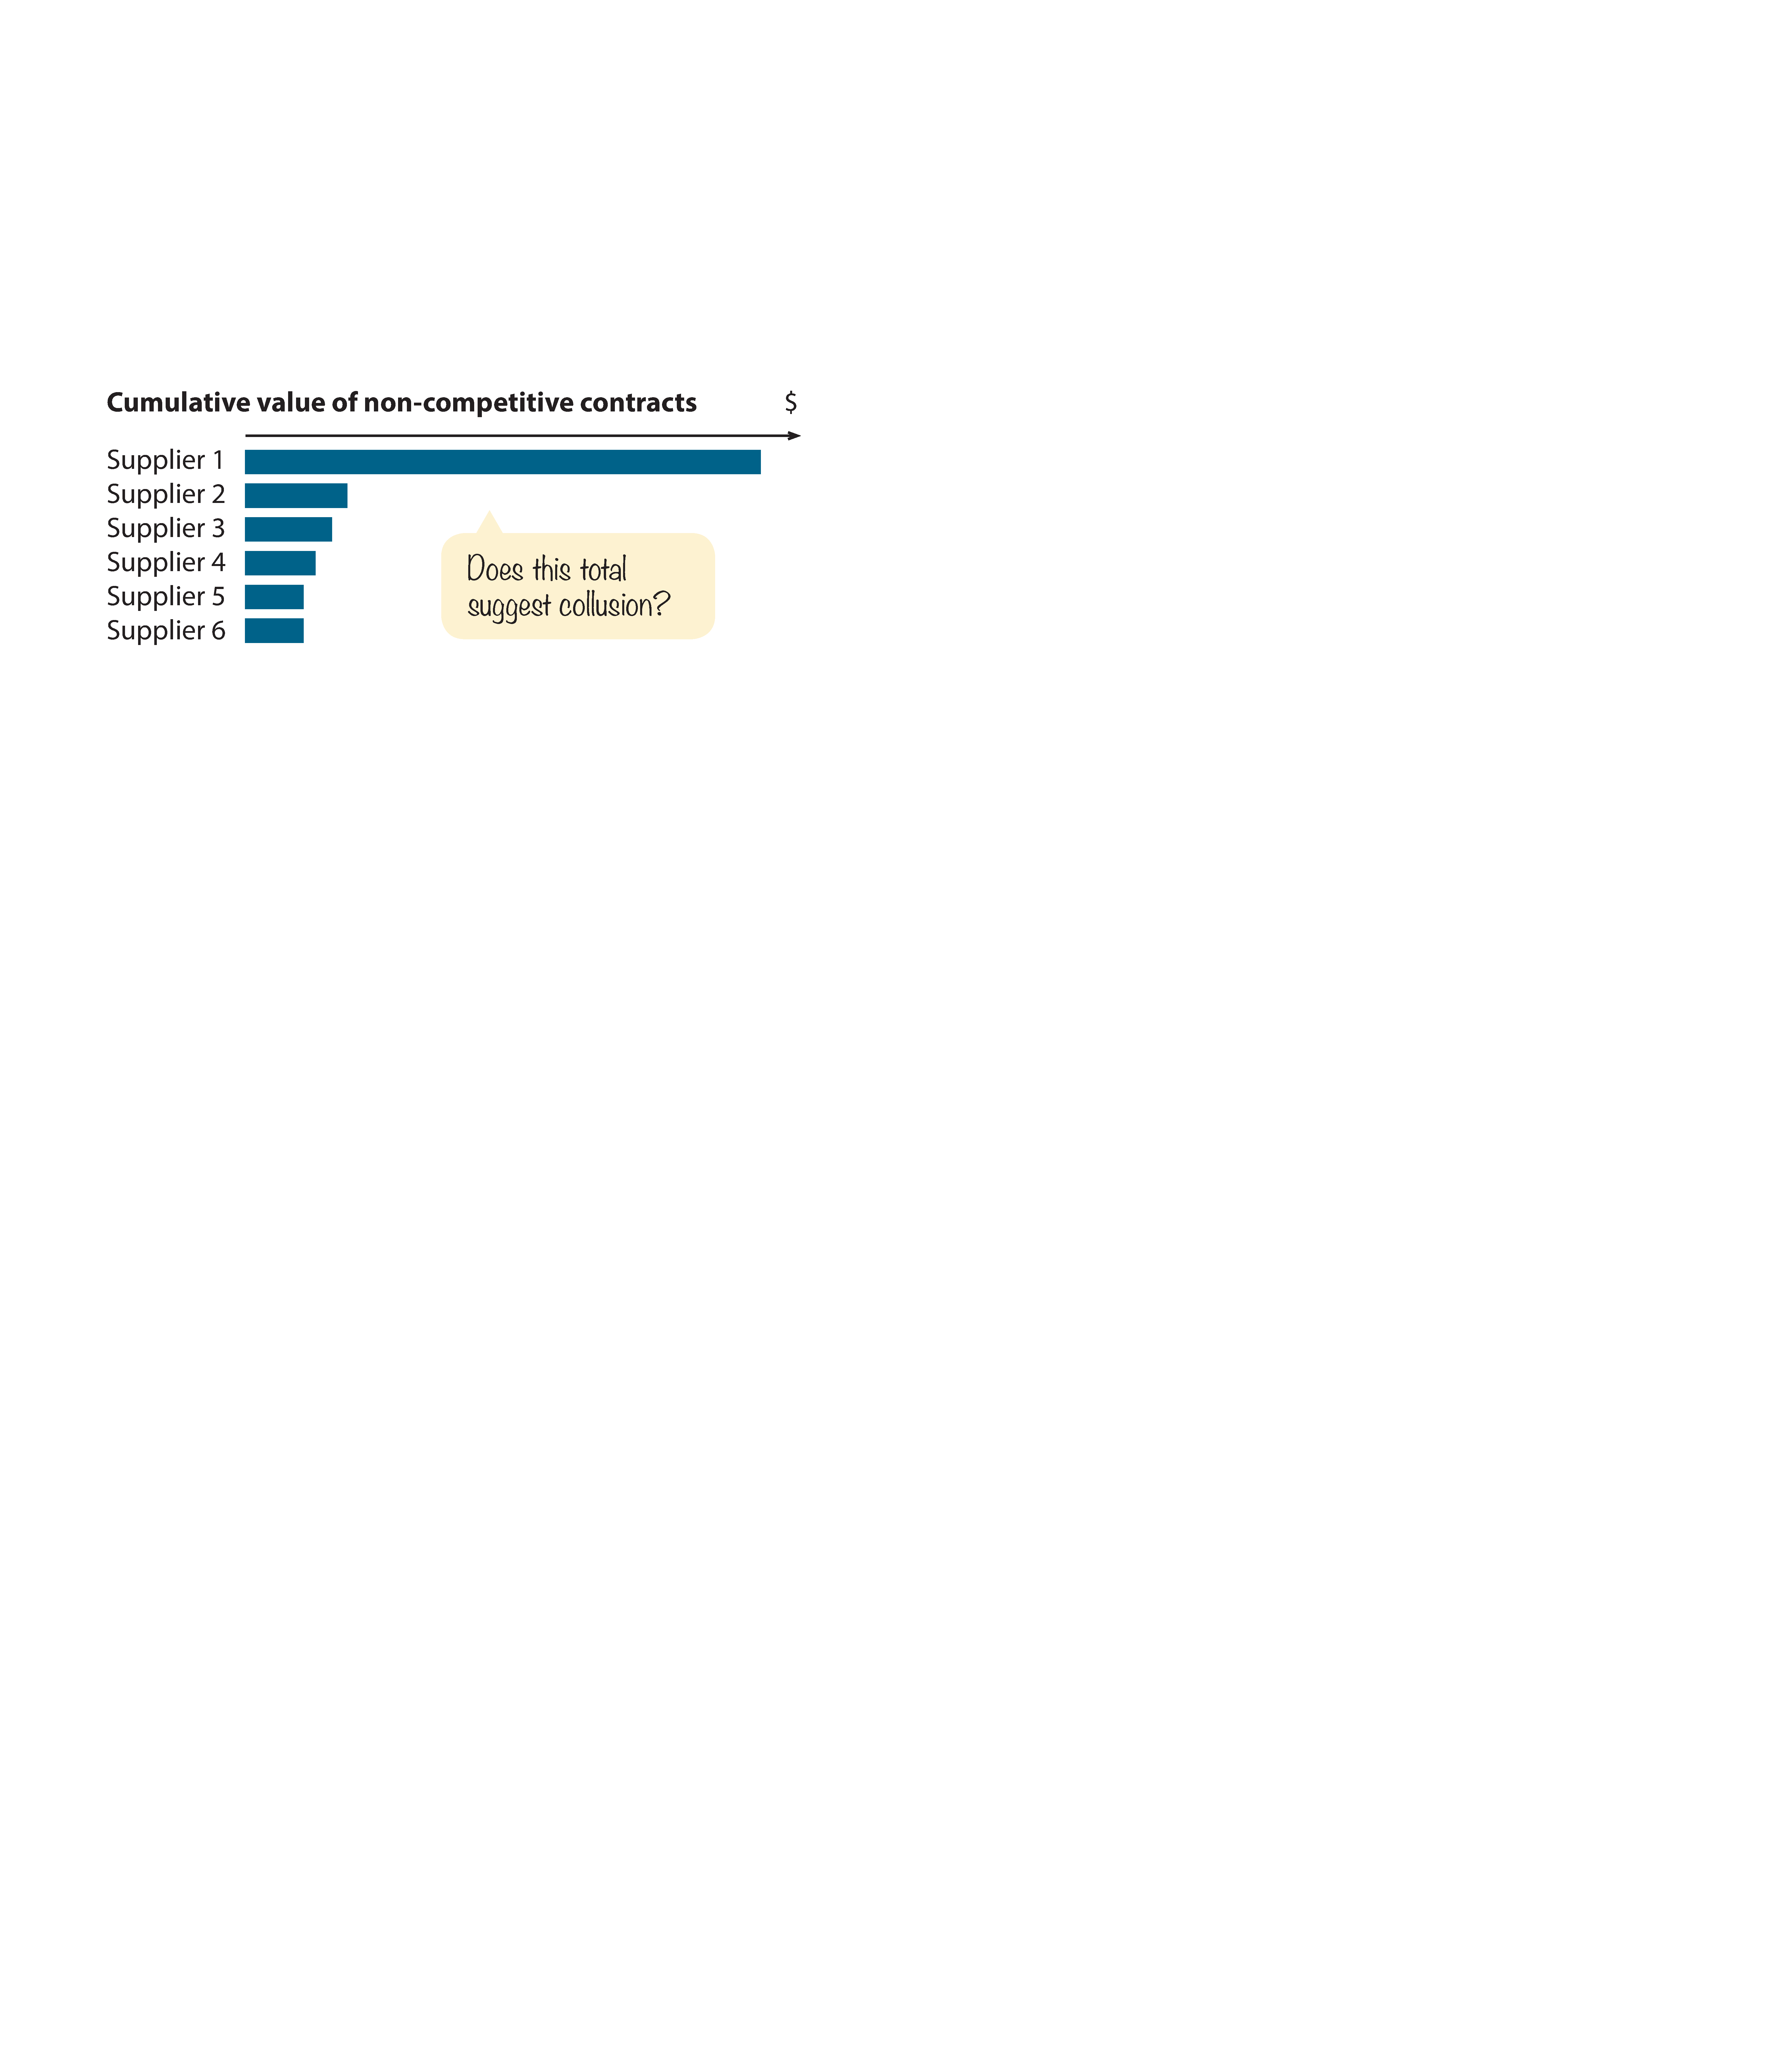
\includegraphics[max width=1\textwidth]{../img/poster_cumulative_value.pdf}
\end{subfigure}
~
\begin{subfigure}[t]{0.5\textwidth}
\caption{Value of Contracts}
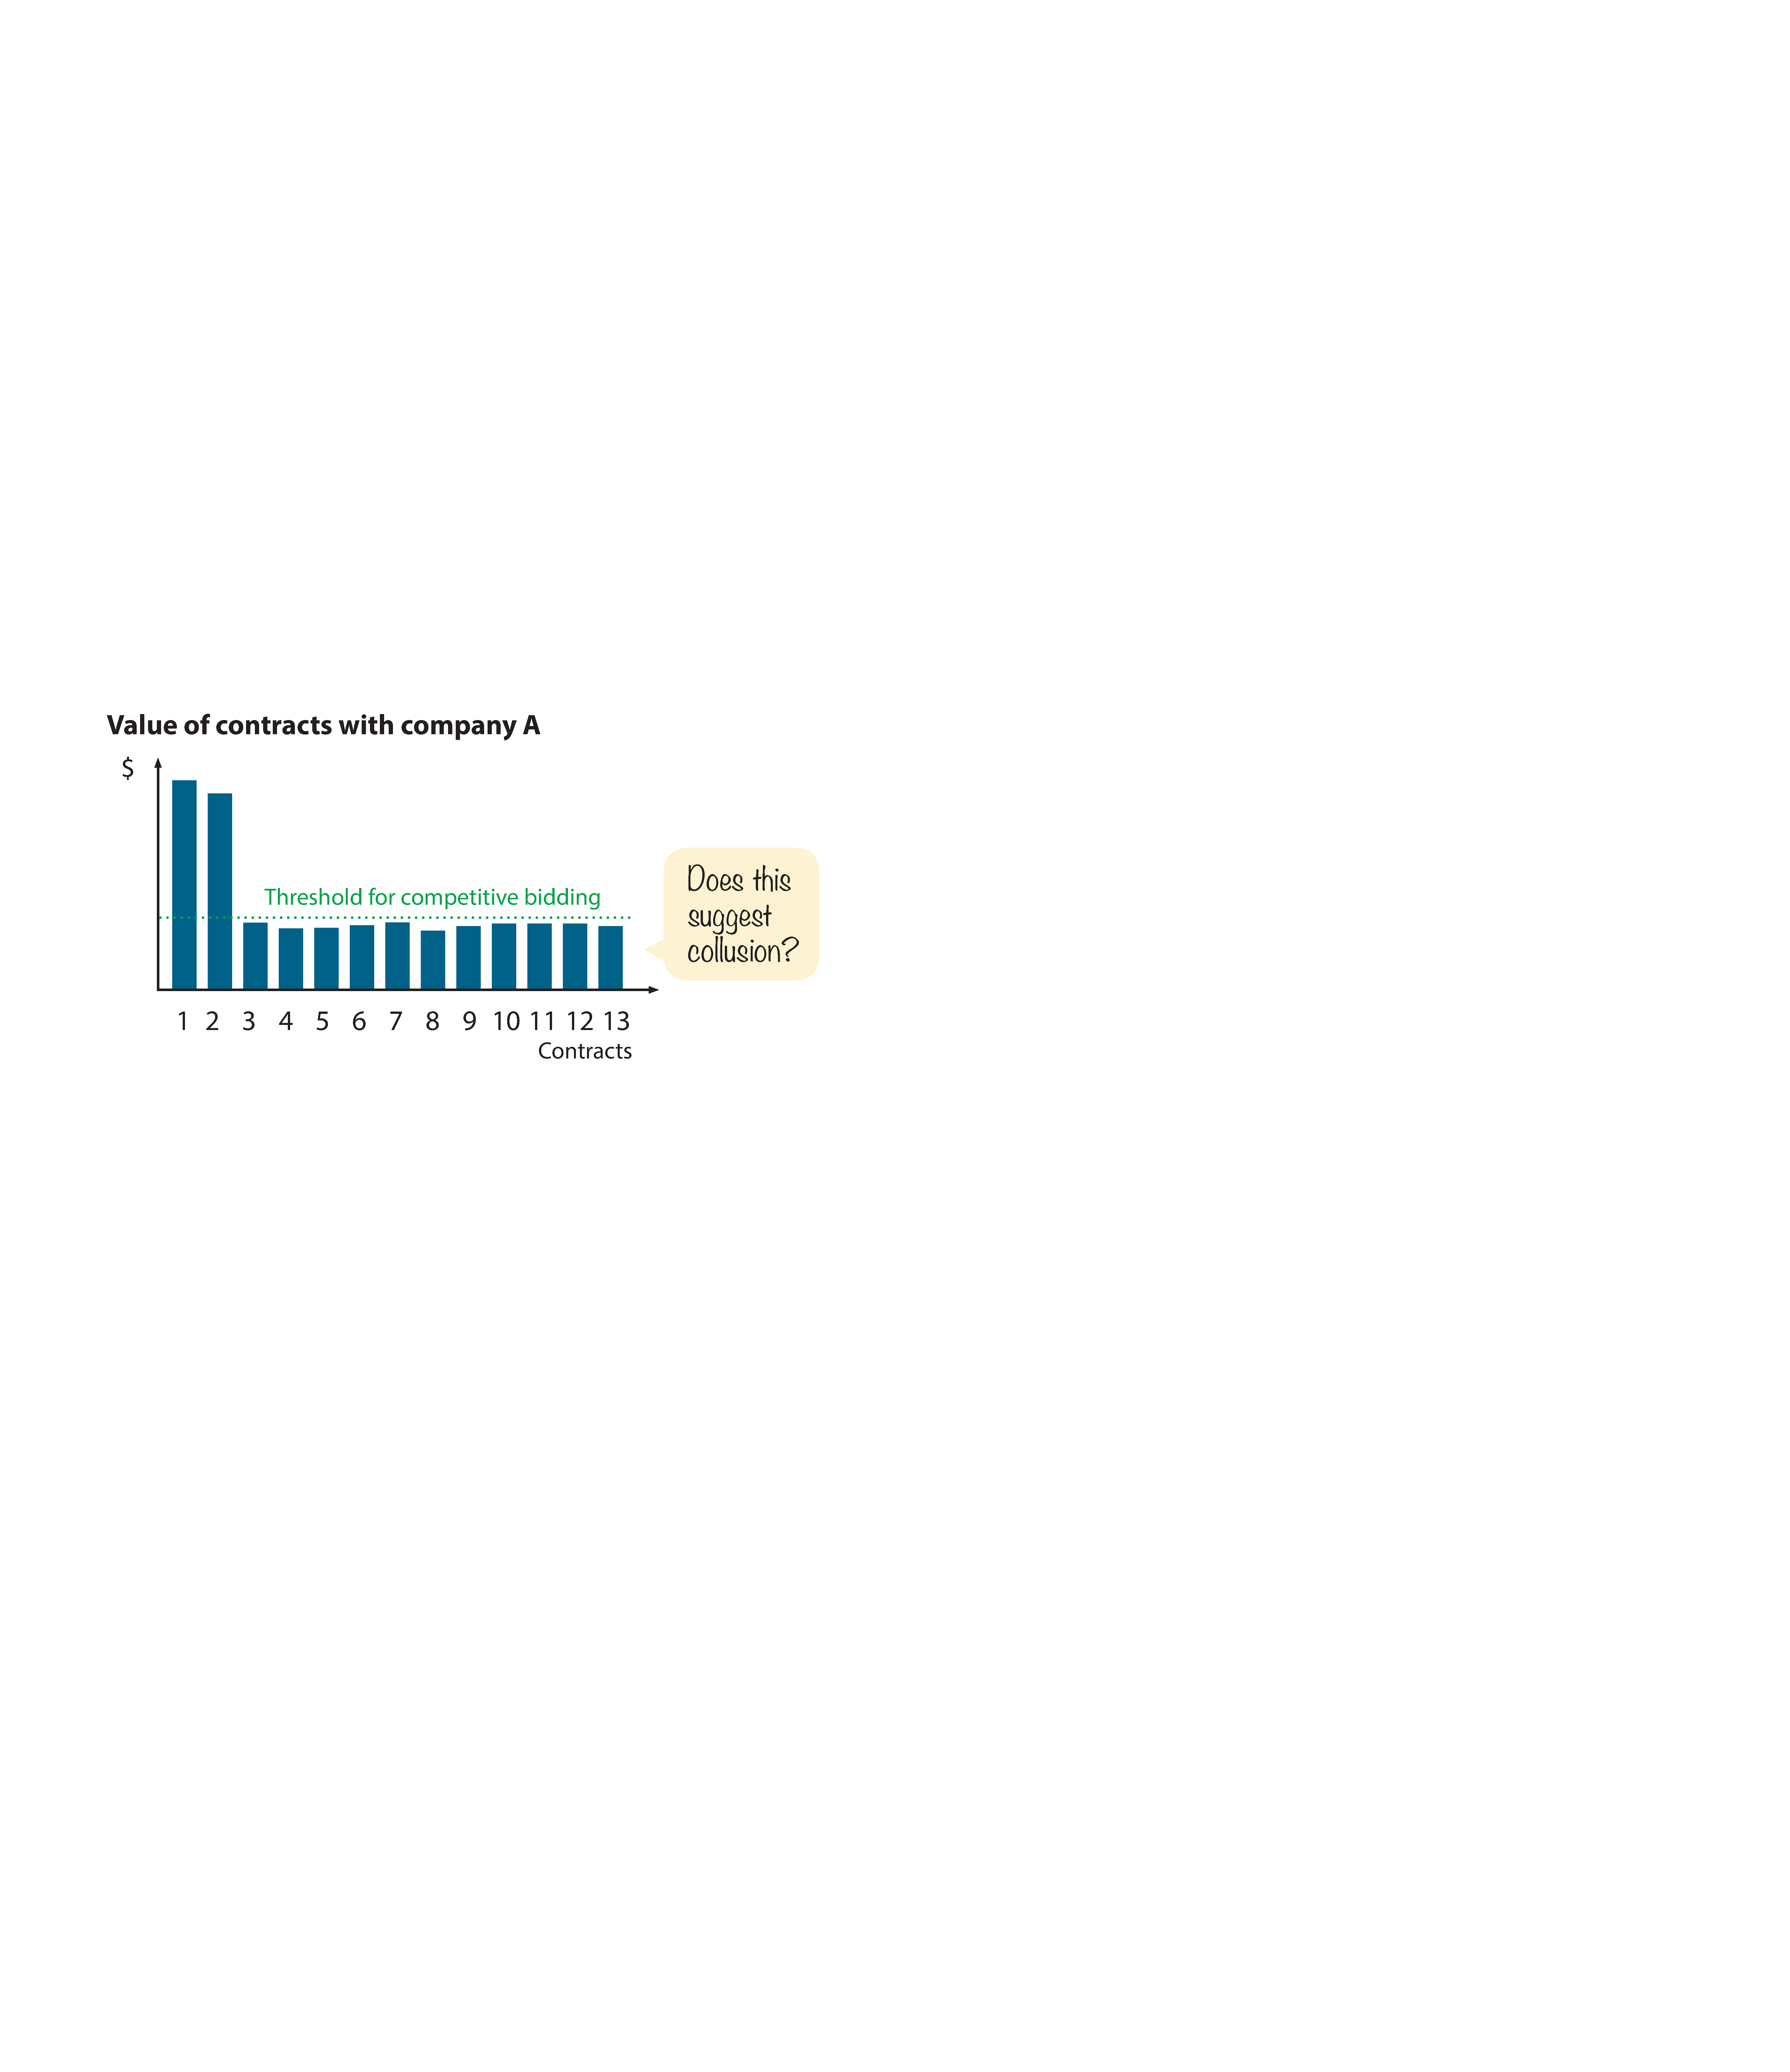
\includegraphics[max width=1\textwidth]{../img/poster_value.pdf}
\end{subfigure}
~
\begin{subfigure}[t]{0.5\textwidth}
\caption{Winning patterns}
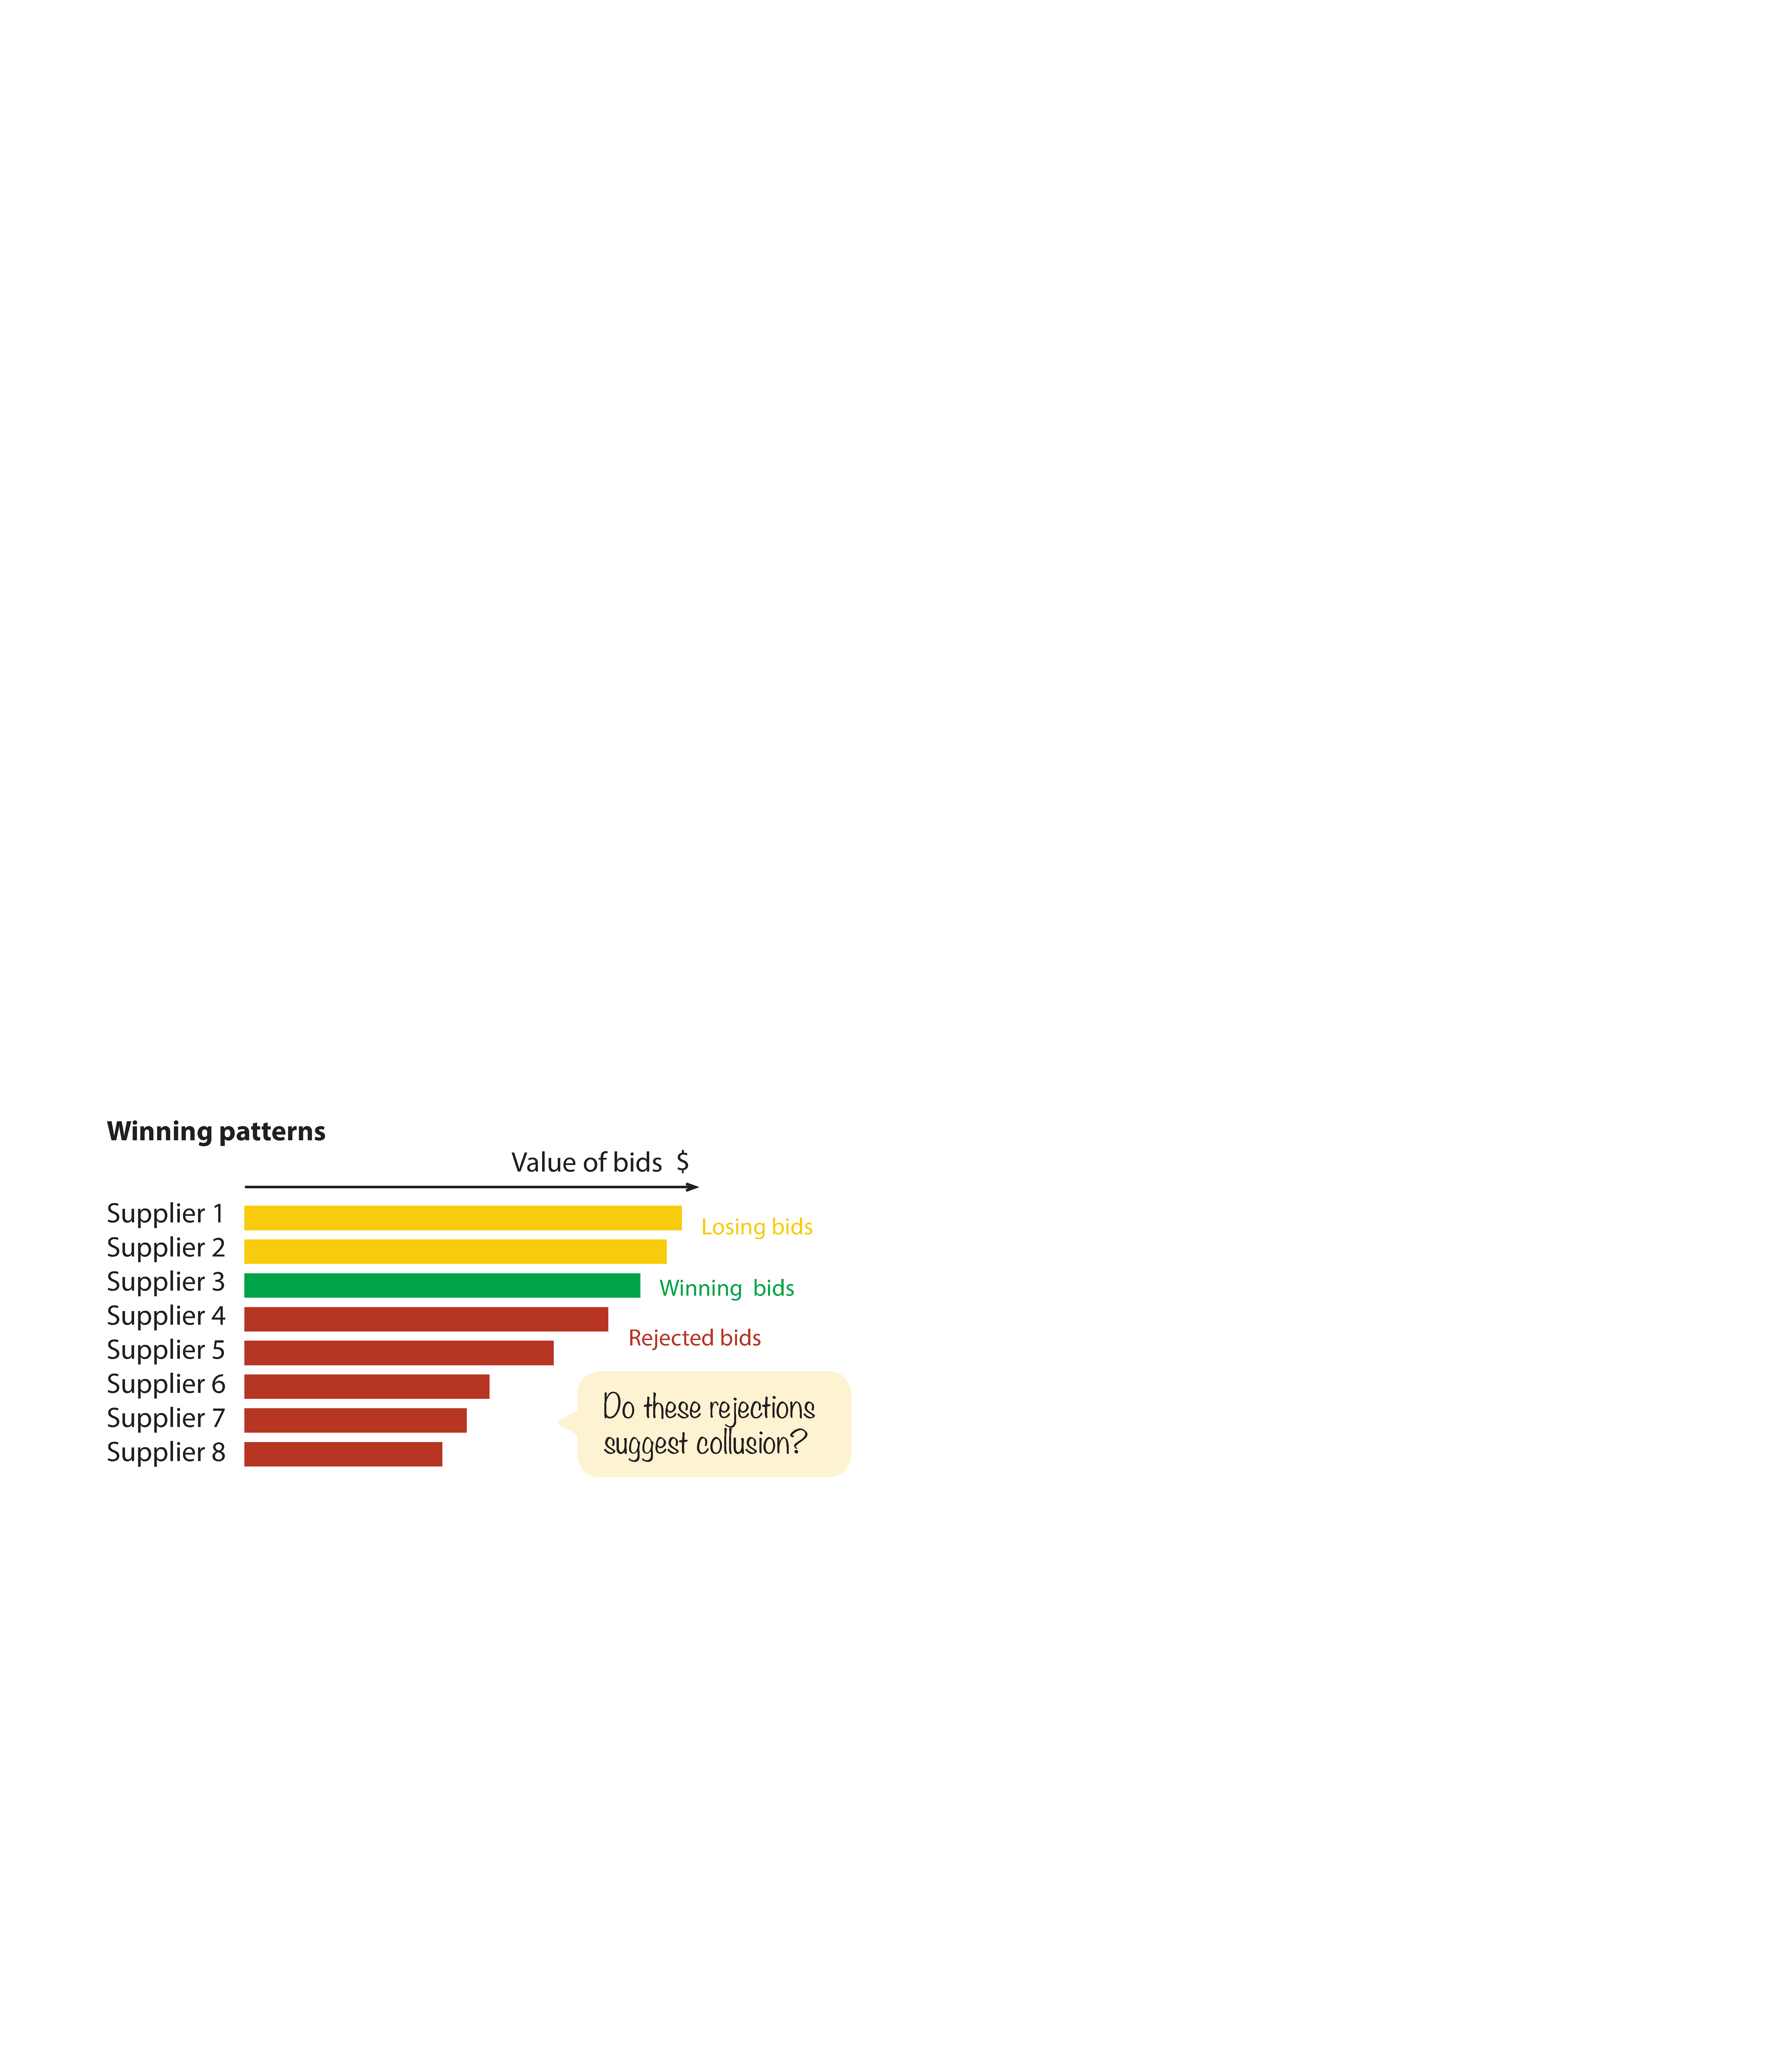
\includegraphics[max width=1\textwidth]{../img/poster_winning_patterns.pdf}
\end{subfigure}
~
\begin{subfigure}[t]{0.5\textwidth}
\caption{Monthly value of non-competitive contracts}
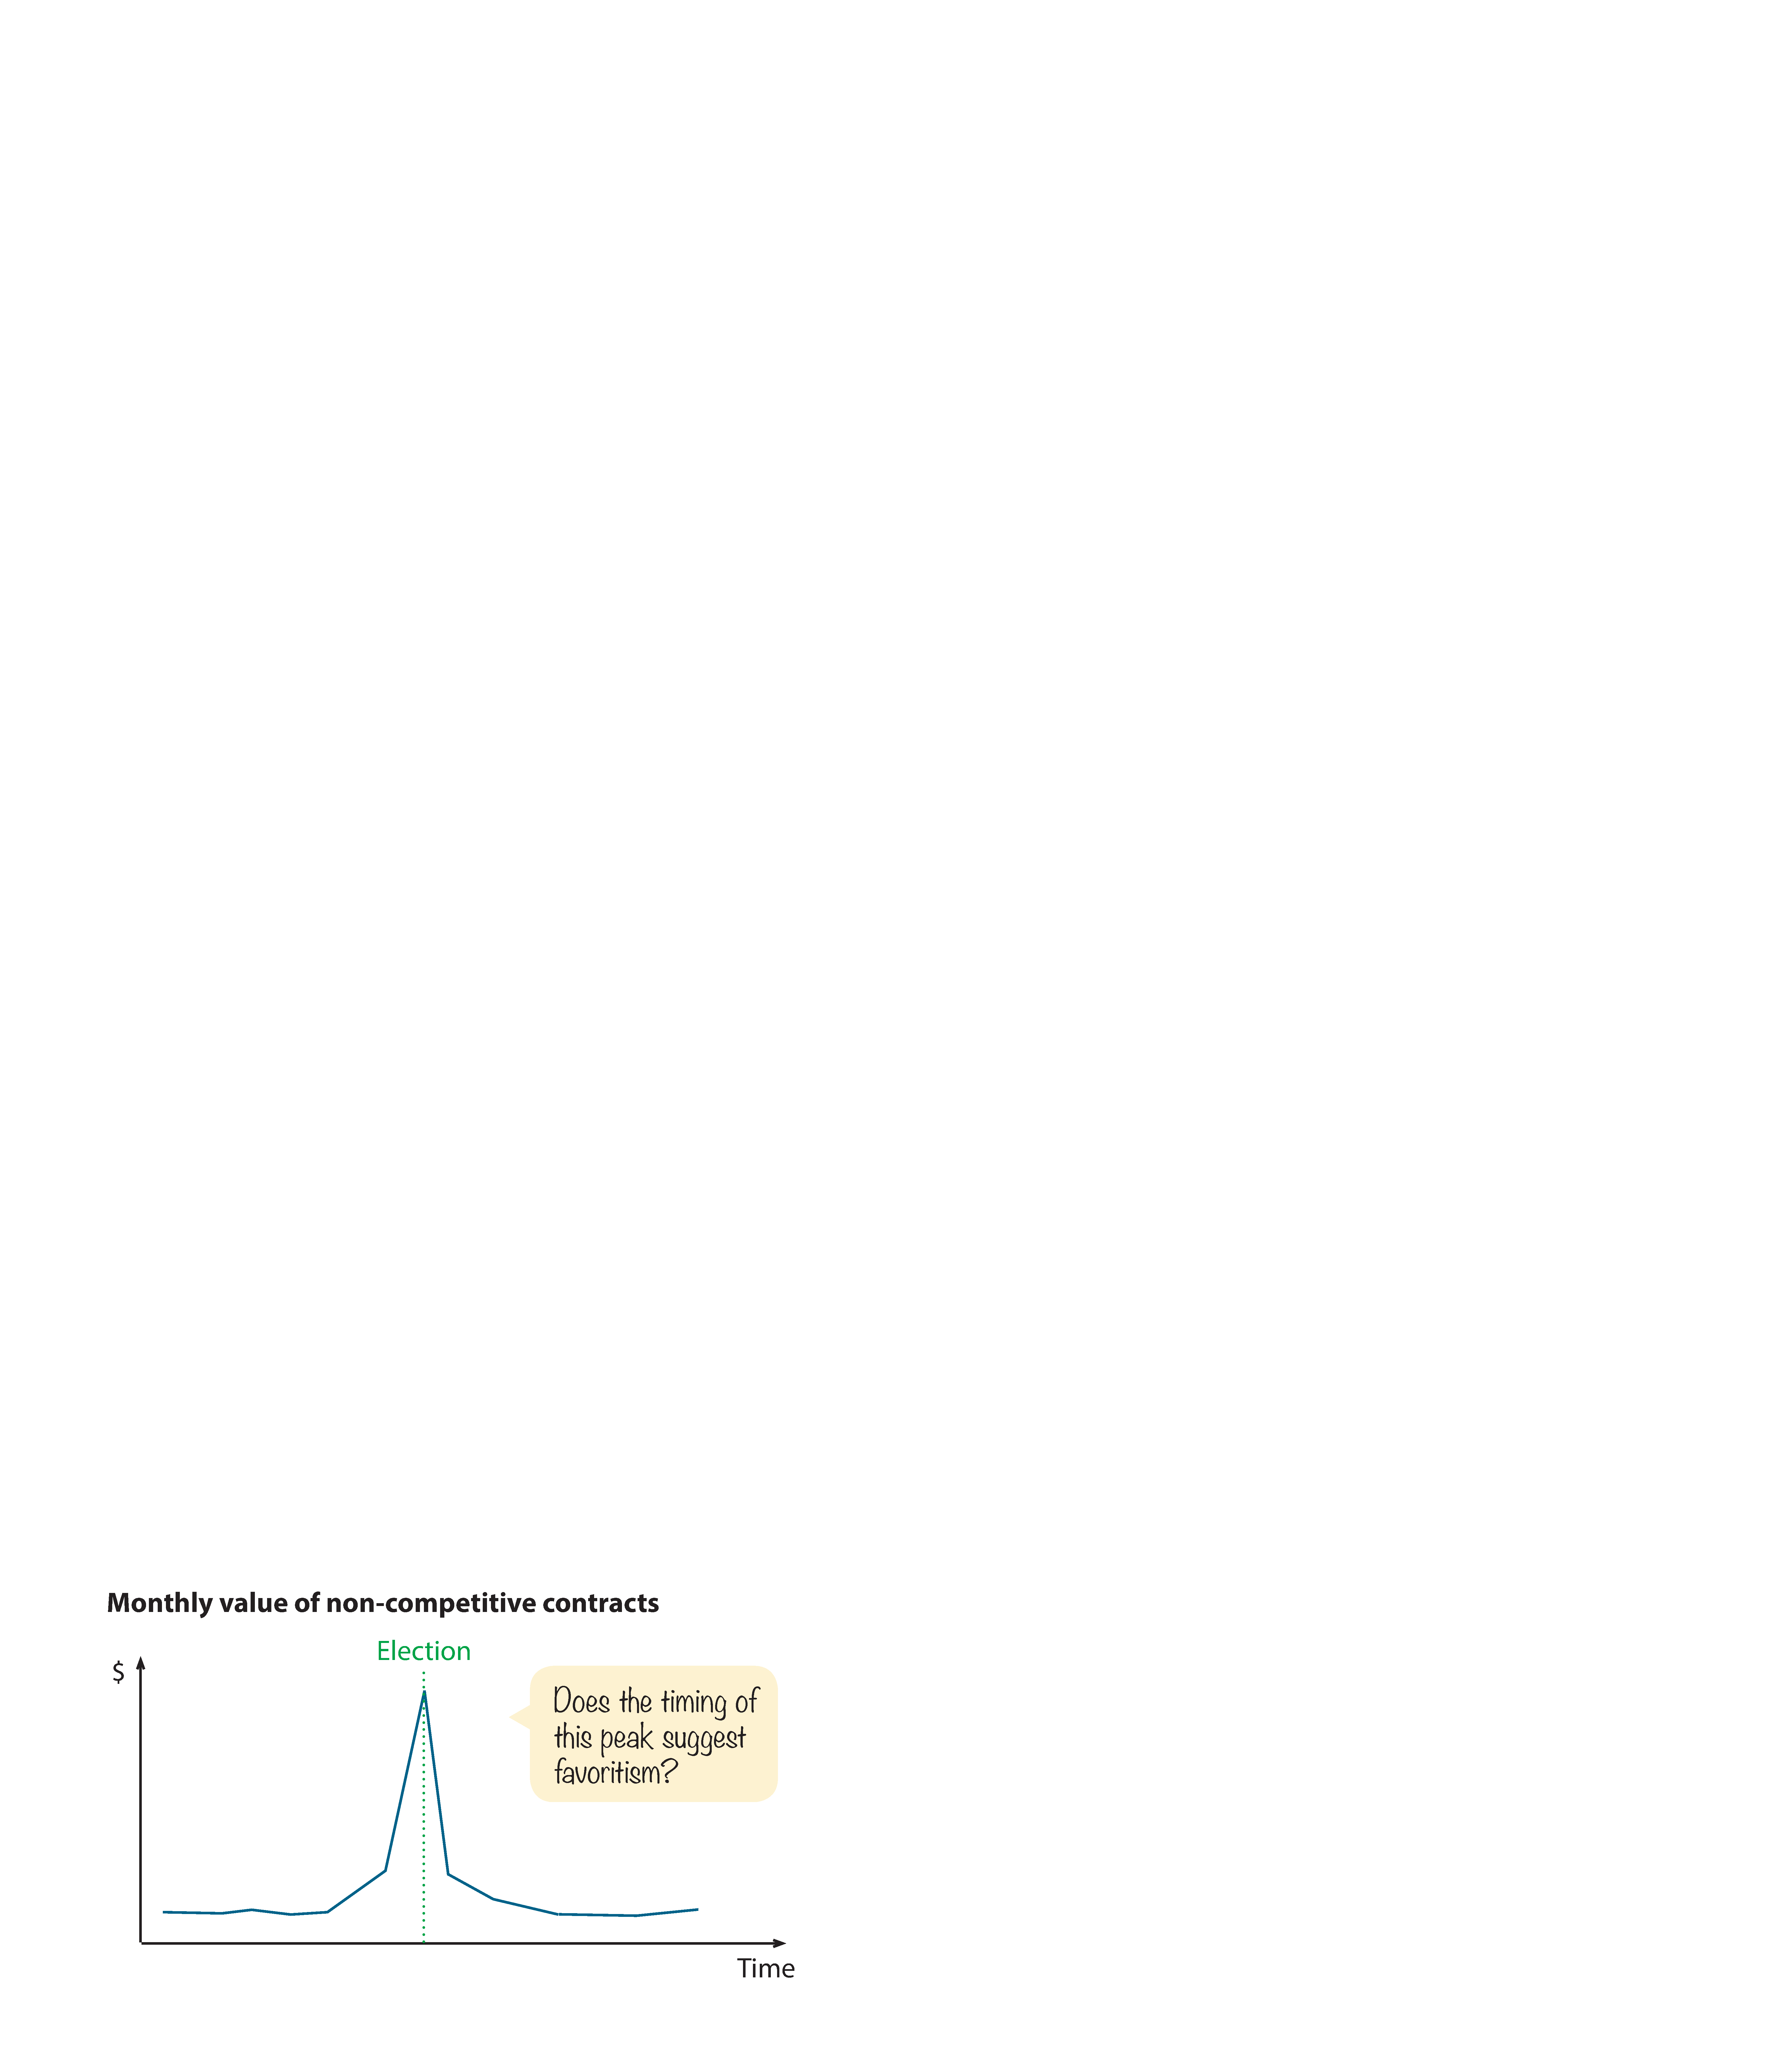
\includegraphics[max width=1\textwidth]{../img/poster_monthly.pdf}
\end{subfigure}
~
\begin{subfigure}[t]{0.5\textwidth}
\caption{Links between companies }
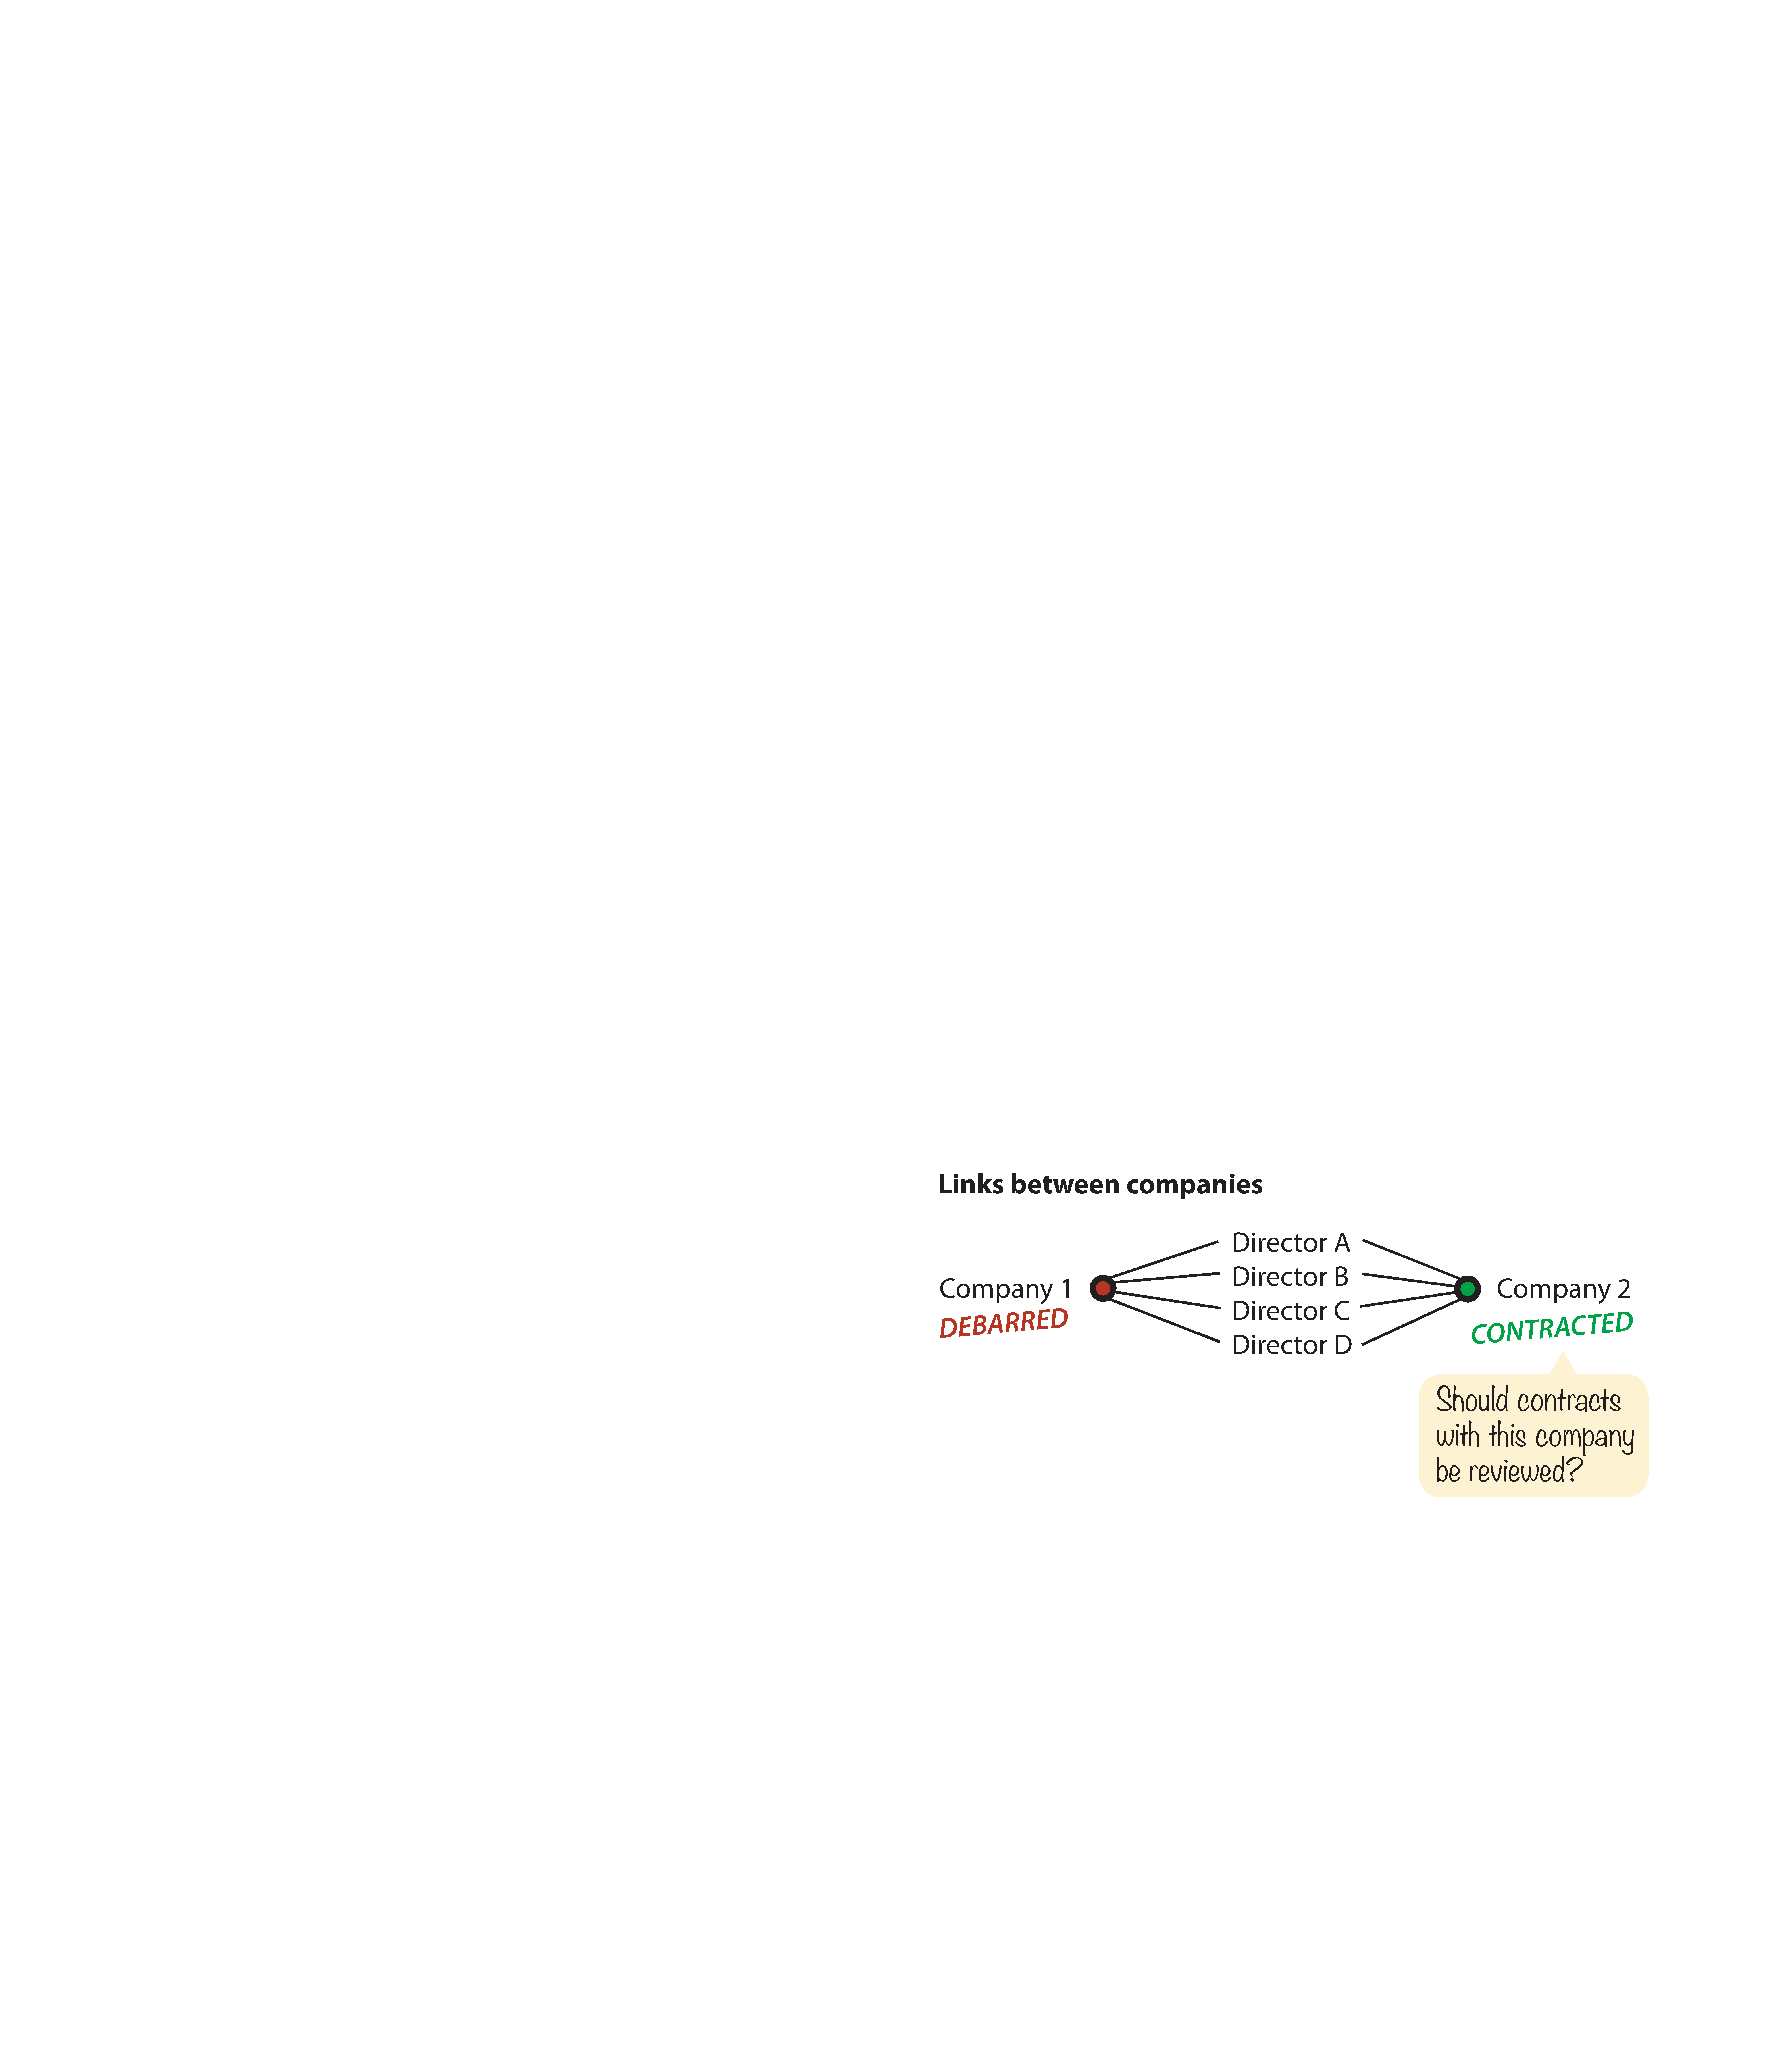
\includegraphics[max width=1\textwidth]{../img/poster_link.pdf}
\end{subfigure}
~
\begin{subfigure}[t]{0.5\textwidth}
\caption{Bidding patterns}
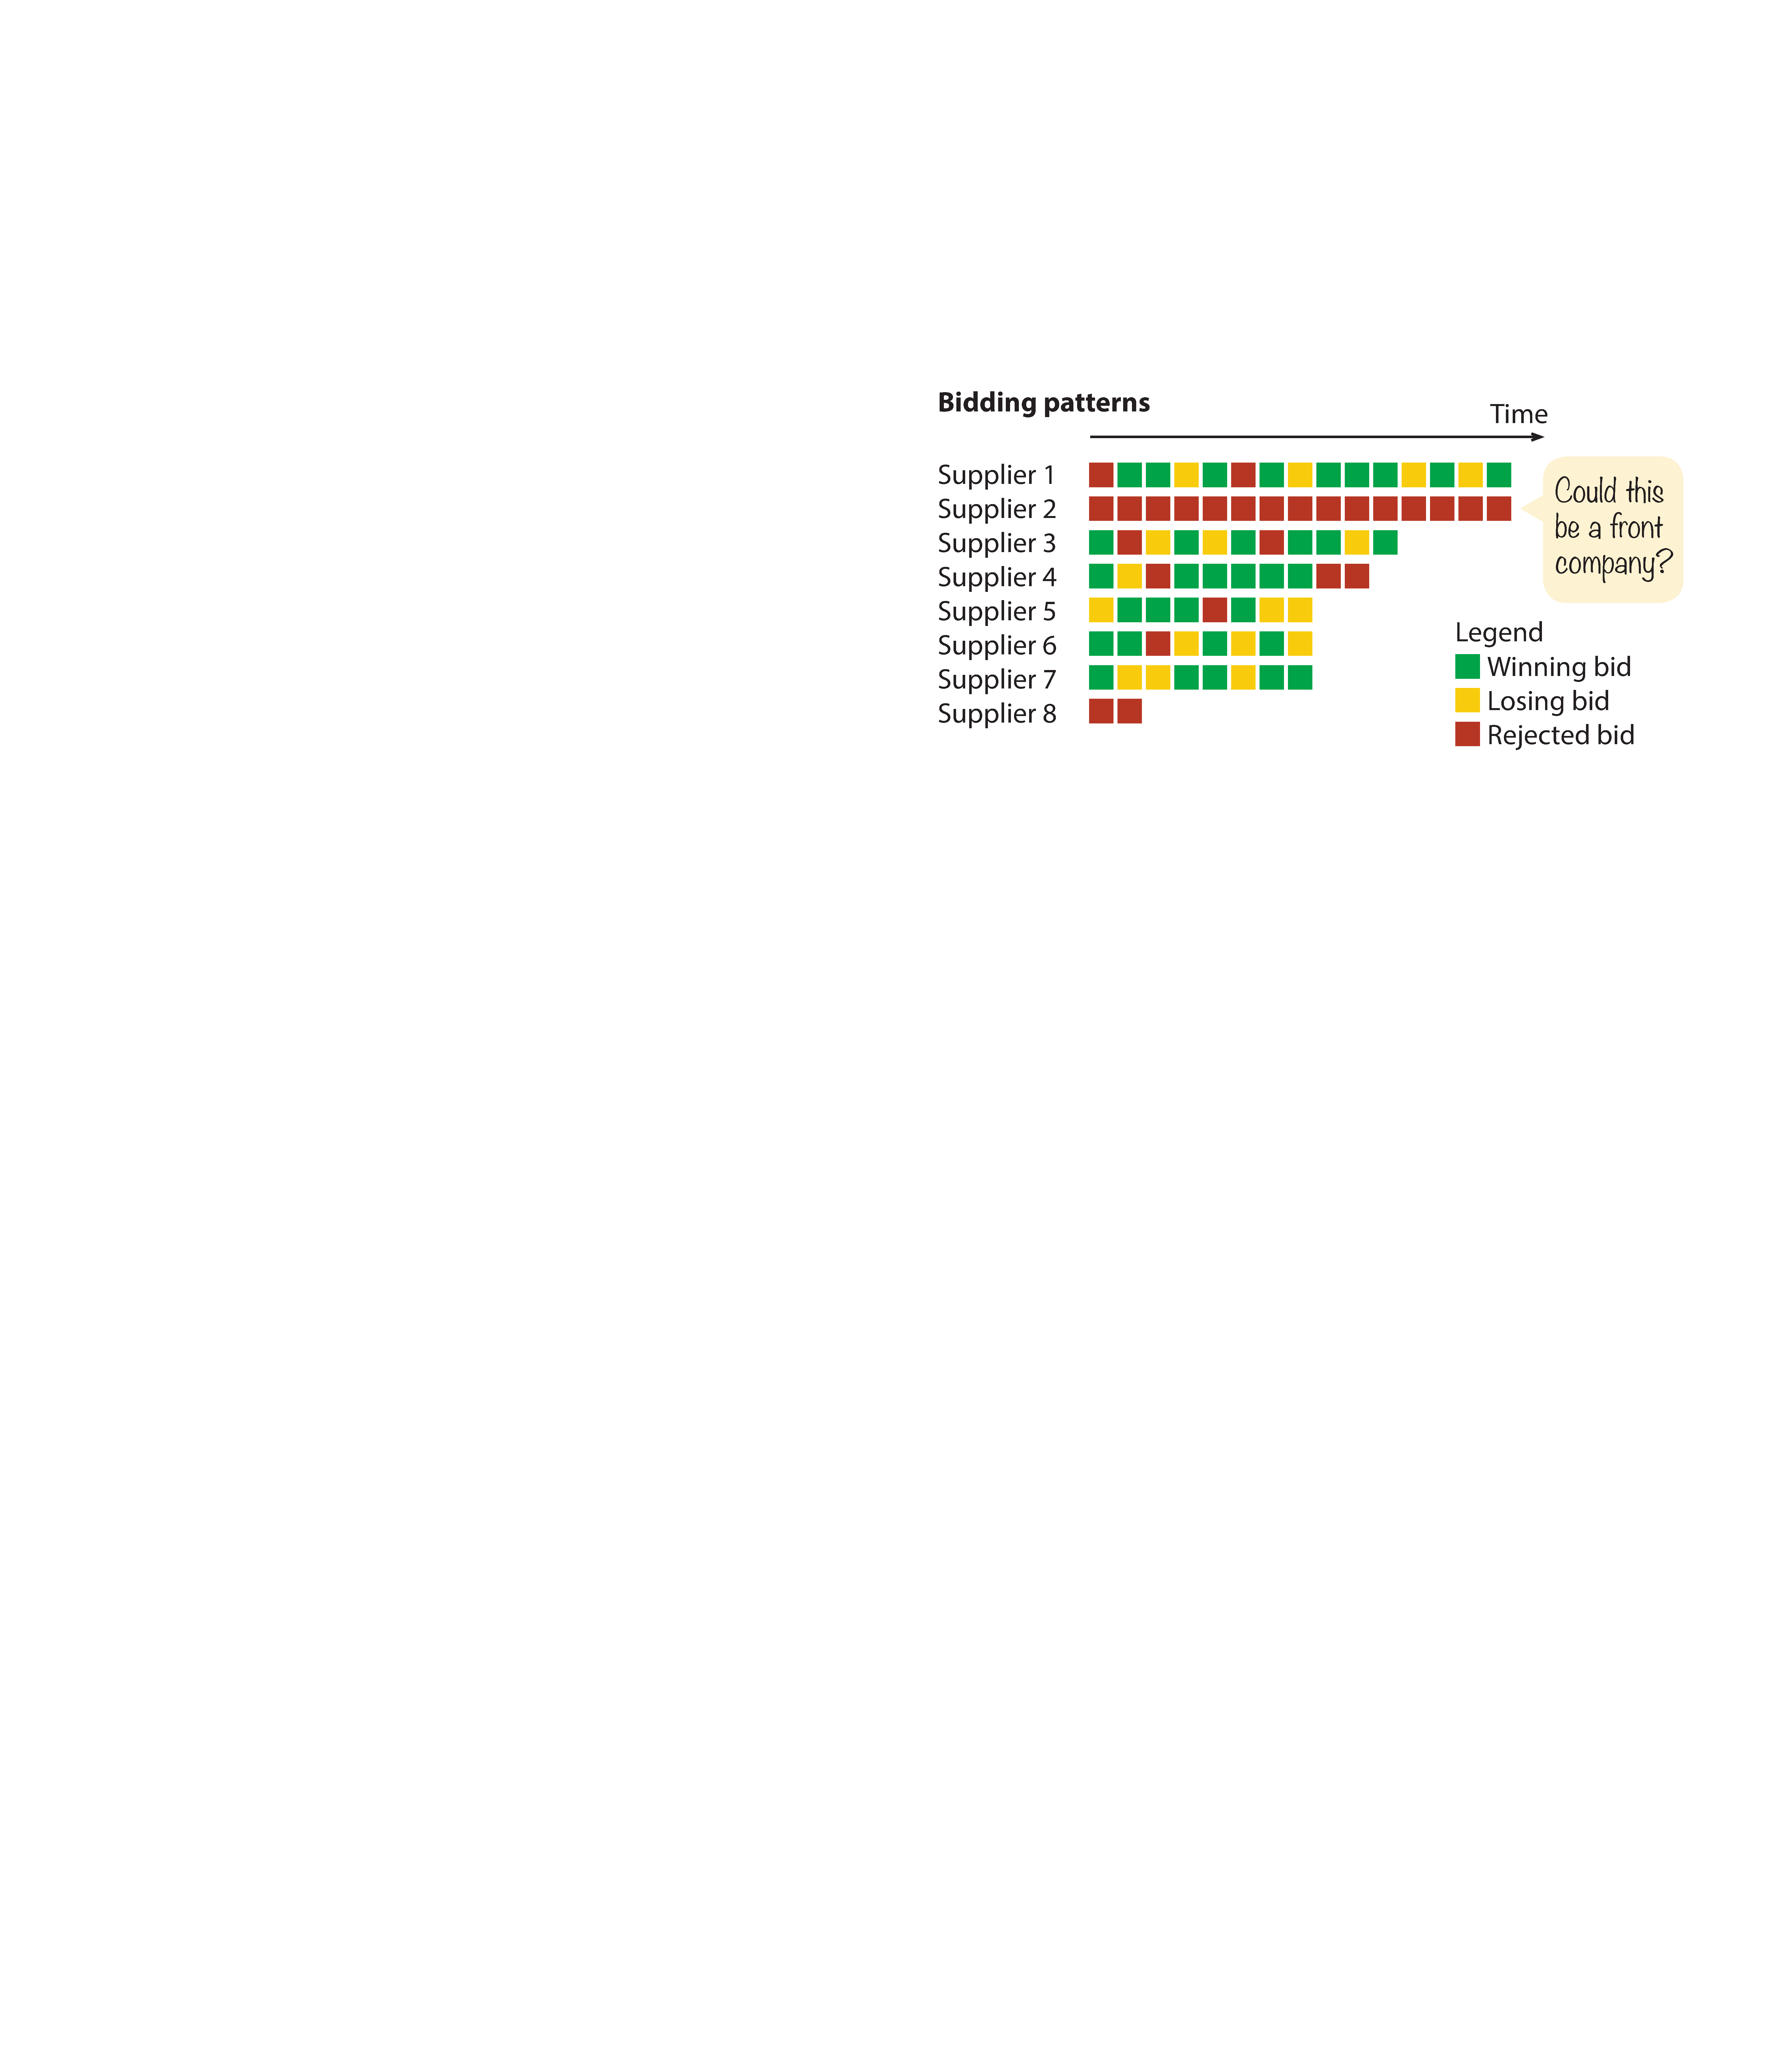
\includegraphics[max width=1\textwidth]{../img/poster_bidding_patt.pdf}
\end{subfigure}

\end{figure}
\clearpage
\begin{figure}[H]
\ContinuedFloat

\begin{subfigure}[t]{0.5\textwidth}
\caption{Bidding patterns}
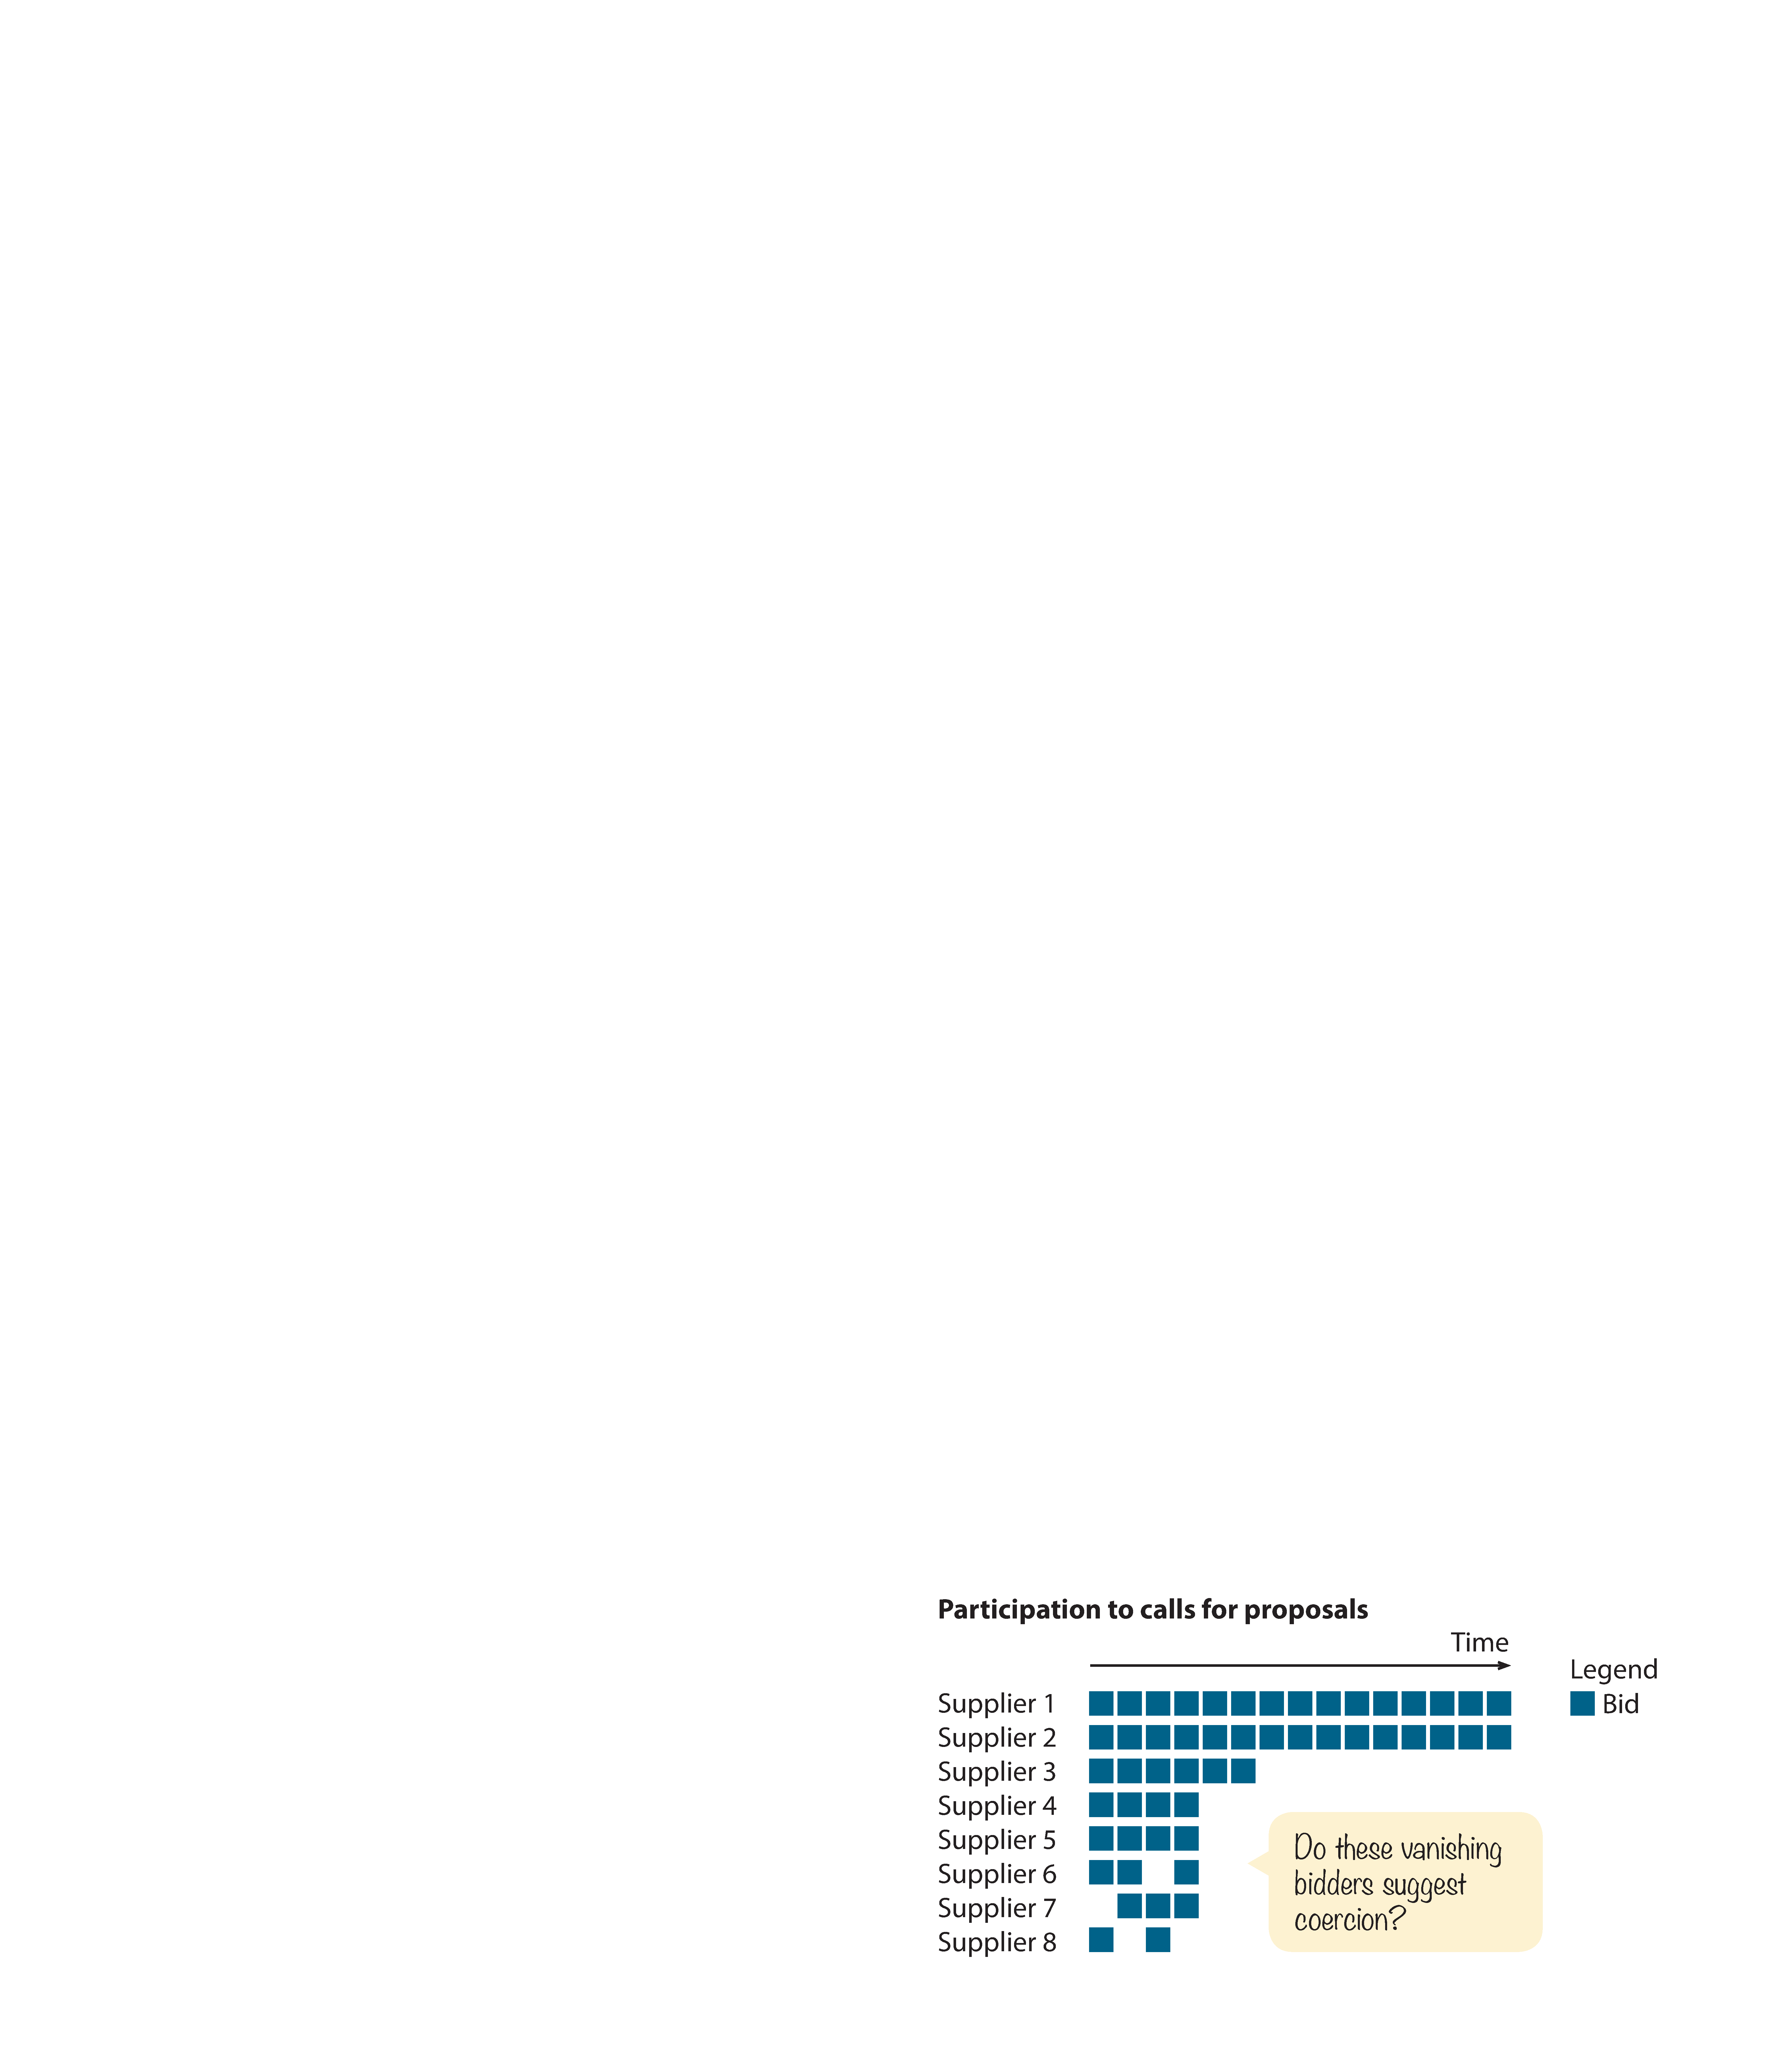
\includegraphics[max width=1\textwidth]{../img/poster_coercion.pdf}
\end{subfigure}
~
\begin{subfigure}[t]{0.5\textwidth}
\caption{Bidding patterns}
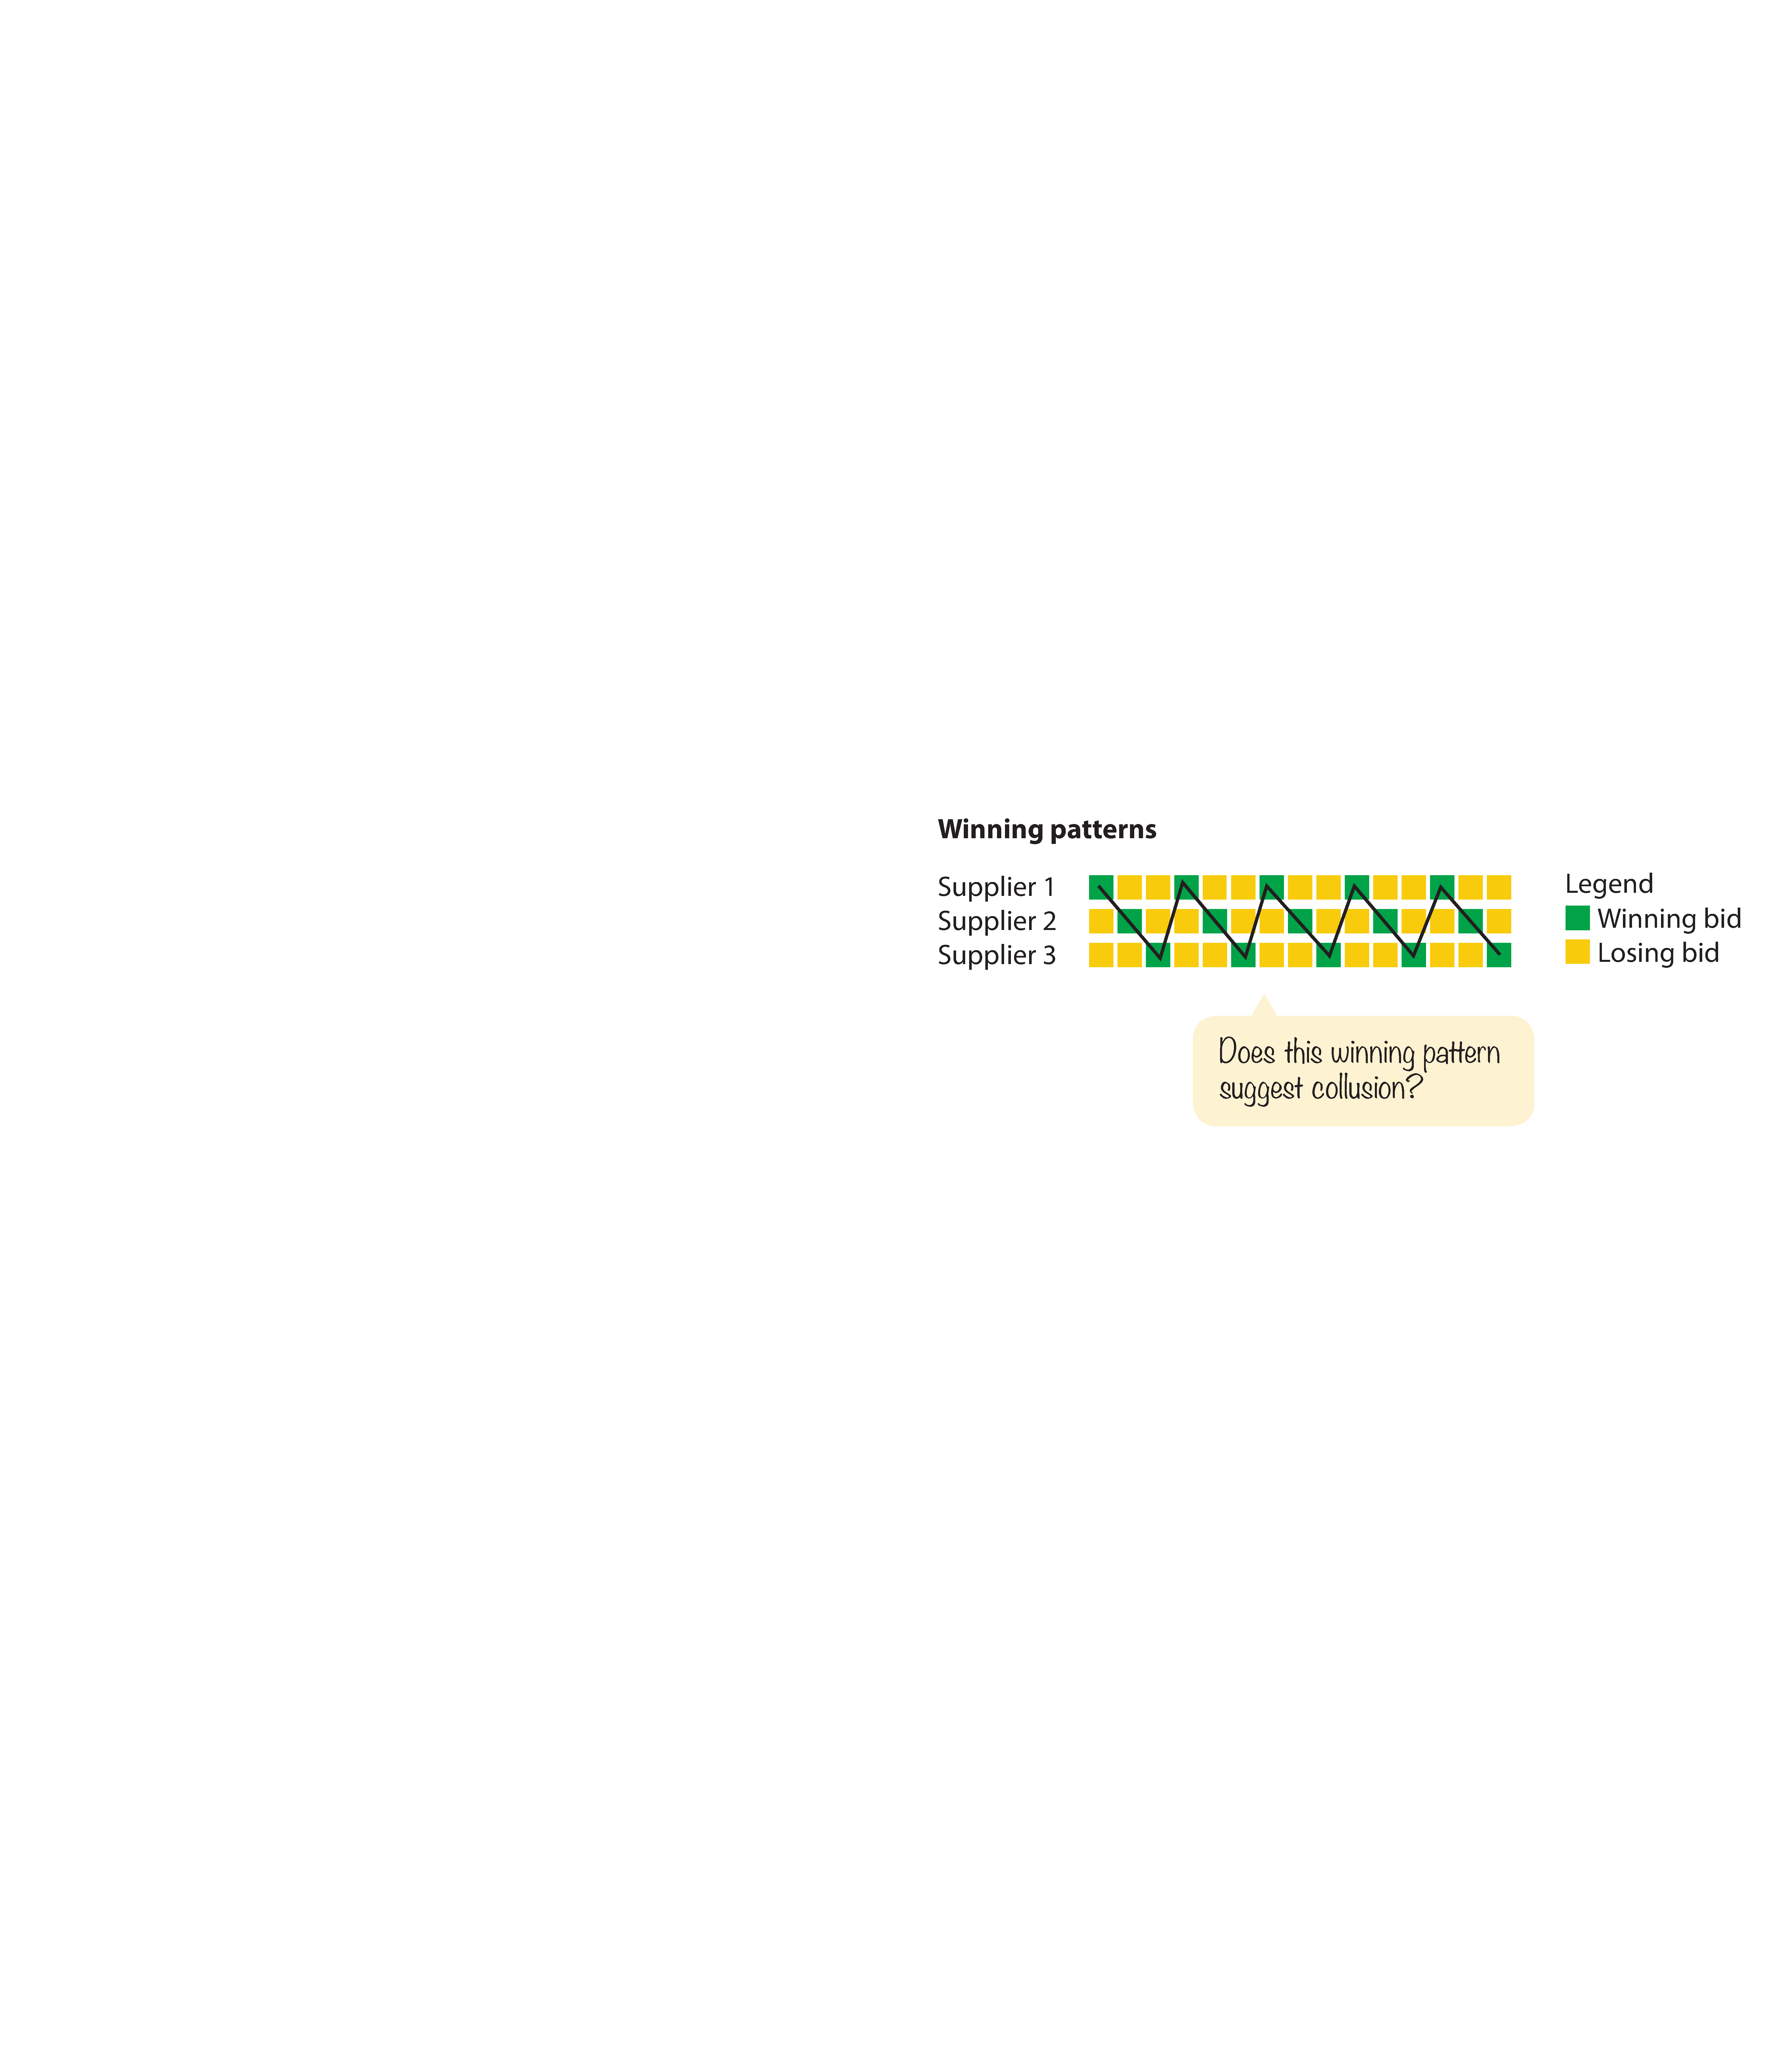
\includegraphics[max width=1\textwidth]{../img/poster_win_pattern.pdf}
\end{subfigure}
\footnotesize{\textbf{Source:} Figures taken from \cite{wb_poster}}
\end{figure}



\section{Report}
Report Suspected Fraud or Corruption


% To Report an Allegation:
% Submit an Online Integrity Complaint Form 
% Download the free Integrity App

% Can INT help me with my concerns?
% If you have an allegation that involves possible fraud, corruption, collusion, coercion and obstruction in World Bank-funded projects and/or against World Bank staff, the World Bank's Integrity Vice Presidency (INT) may be able to help address your concerns. Click here for definitions and examples.

% How do I report?
% The Integrity Complaint Form is the best way to send a report to INT. When you click on the link to the Form, you will be taken to a secure and confidential third-party website that is managed by INT. You will need to provide basic information regarding your allegations and a detailed summary of your concerns. There are available “Guide Questions” to help you fill out the Form. You also have the option to upload supporting documents after submitting the Form.

% The Integrity App can also be used to provide information to INT, as appropriate.

% Why should I report a concern?
% Our investigations are primarily based upon the allegations we receive, so it is extremely important that those people who are involved in activities supported by World Bank Group funds take the initiative to report suspected fraud or corruption.

% When should I expect a response?
% You will receive an automated response with a reference number when you submit a report to INT using the Integrity Complaint Form and the Integrity App.

% If your report pertains to fraud, corruption, collusion, coercion and obstruction involving World Bank-funded projects or World Bank staff, someone from INT will contact you directly using the contact information that you have provided.

 	
% Can I remain anonymous?

% Yes. The World Bank will still review your complaint even if you wish to remain anonymous. However, you still will need to provide INT with at least an email address to contact you for additional information or clarification.

% Is my report confidential?
% Yes. All information provided to INT is confidential. We will not disclose information that may reveal your identity without your consent unless the World Bank is required to do so by law.

% Advance Fee Fraud Scams
% The World Bank's name is often used as part of an illicit scam known as Advance Fee Fraud (AFF). If you receive a message with one or more of the following, please be aware that you may have been a victim of an AFF scam:

% --You have won something and your prize money is in an account with some claimed affiliation to  the World Bank

% --You have inherited some money that can be withdrawn from an account with some claimed affiliation to the World Bank

% --A person or organization claiming to be affiliated with the World Bank is asking money, personal details and/or banking information in exchange for a job, a personal loan, an ATM/credit card, etc.


% The World Bank does not send these types of messages. To protect yourself, do NOT reply to the message. Do NOT send your banking details, personal information, and any money to anyone claiming to be from the World Bank. The World Bank cannot assist you in recovering any lost funds.

% If you believe that you may have been a victim of AFF scams, please contact your local authorities. Learn more.

% Other Concerns
% Requests for project information, documents and data, statistics and publications: Access to Information

% Job applications: www.worldbank.org/jobs

% Verification of employment for World Bank Group employees: Contact World Bank's Human Resources Service Center at (202) 473-2222 or hrservicecenter@worldbank.org













